\documentclass[a4paper, 10pt]{article}
% All LaTeX documents including
% tikz() output must use this
% package!
\usepackage[margin=2.5cm]{geometry}
\usepackage{tikz}
\usepackage{pdflscape}

\newcommand{\insertplot}[2]{
  \begin{figure}[!ht]
    \centering
    \input{#1}
    \caption{#2}
  \end{figure}
}

\begin{document}

% \begin{landscape}
%   \begin{figure}[!h]
%     \centering
%     % Created by tikzDevice version 0.8.1 on 2015-11-03 22:36:52
% !TEX encoding = UTF-8 Unicode
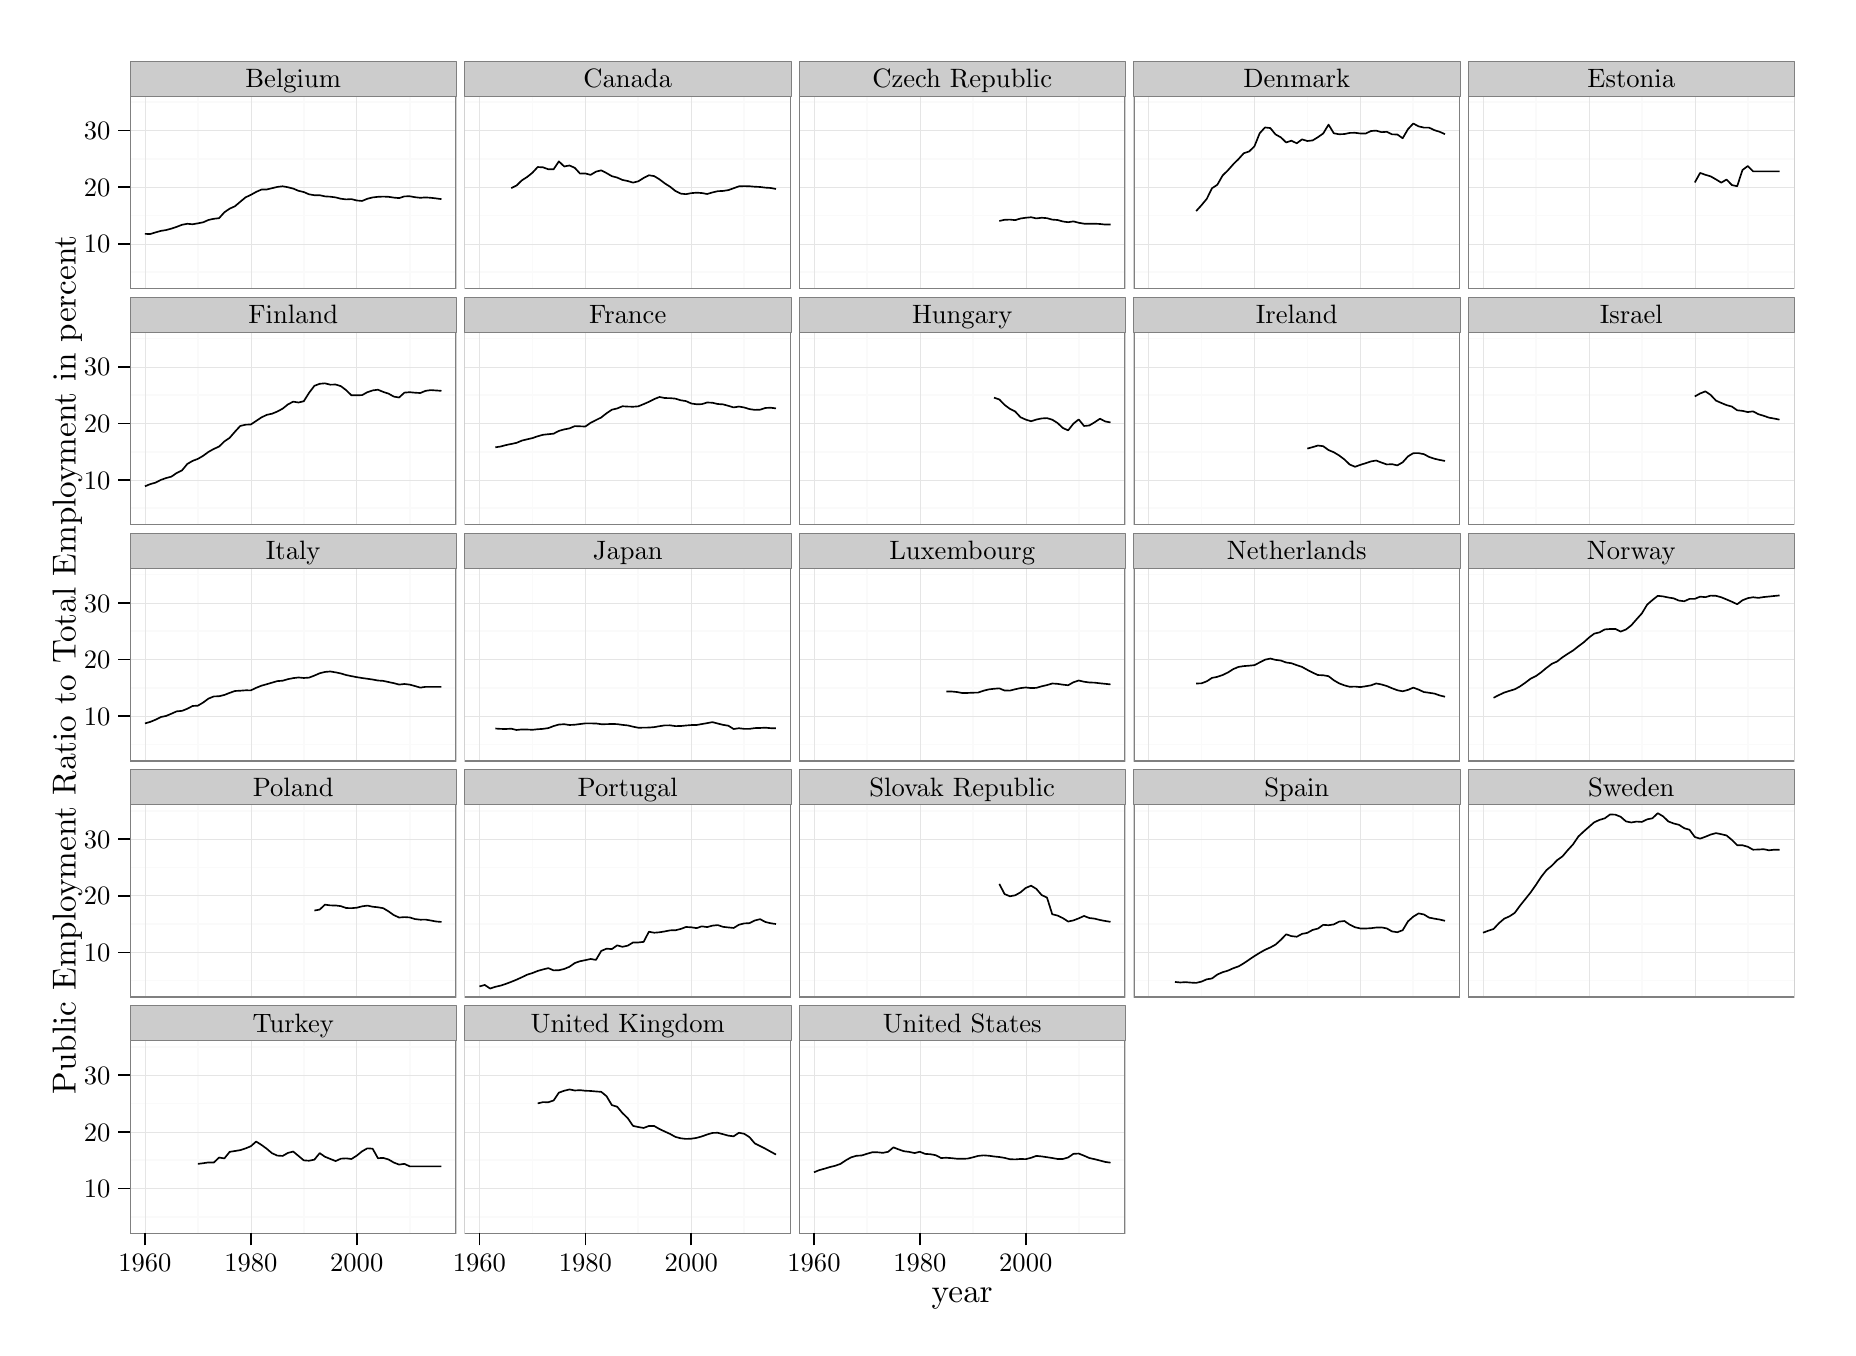
\begin{tikzpicture}[x=1pt,y=1pt]
\definecolor{fillColor}{RGB}{255,255,255}
\path[use as bounding box,fill=fillColor,fill opacity=0.00] (0,0) rectangle (650.43,469.75);
\begin{scope}
\path[clip] (  0.00,  0.00) rectangle (650.43,469.75);
\definecolor{drawColor}{RGB}{255,255,255}
\definecolor{fillColor}{RGB}{255,255,255}

\path[draw=drawColor,line width= 0.6pt,line join=round,line cap=round,fill=fillColor] (  0.00,  0.00) rectangle (650.43,469.76);
\end{scope}
\begin{scope}
\path[clip] ( 37.02,375.38) rectangle (154.88,445.08);
\definecolor{fillColor}{RGB}{255,255,255}

\path[fill=fillColor] ( 37.02,375.38) rectangle (154.88,445.08);
\definecolor{drawColor}{gray}{0.98}

\path[draw=drawColor,line width= 0.6pt,line join=round] ( 37.02,381.41) --
	(154.88,381.41);

\path[draw=drawColor,line width= 0.6pt,line join=round] ( 37.02,401.86) --
	(154.88,401.86);

\path[draw=drawColor,line width= 0.6pt,line join=round] ( 37.02,422.31) --
	(154.88,422.31);

\path[draw=drawColor,line width= 0.6pt,line join=round] ( 37.02,442.77) --
	(154.88,442.77);

\path[draw=drawColor,line width= 0.6pt,line join=round] ( 61.51,375.38) --
	( 61.51,445.08);

\path[draw=drawColor,line width= 0.6pt,line join=round] ( 99.78,375.38) --
	( 99.78,445.08);

\path[draw=drawColor,line width= 0.6pt,line join=round] (138.05,375.38) --
	(138.05,445.08);
\definecolor{drawColor}{gray}{0.90}

\path[draw=drawColor,line width= 0.2pt,line join=round] ( 37.02,391.63) --
	(154.88,391.63);

\path[draw=drawColor,line width= 0.2pt,line join=round] ( 37.02,412.09) --
	(154.88,412.09);

\path[draw=drawColor,line width= 0.2pt,line join=round] ( 37.02,432.54) --
	(154.88,432.54);

\path[draw=drawColor,line width= 0.2pt,line join=round] ( 42.38,375.38) --
	( 42.38,445.08);

\path[draw=drawColor,line width= 0.2pt,line join=round] ( 80.65,375.38) --
	( 80.65,445.08);

\path[draw=drawColor,line width= 0.2pt,line join=round] (118.91,375.38) --
	(118.91,445.08);
\definecolor{drawColor}{RGB}{0,0,0}

\path[draw=drawColor,line width= 0.6pt,line join=round] ( 42.38,395.24) --
	( 44.29,395.18) --
	( 46.20,395.77) --
	( 48.12,396.31) --
	( 50.03,396.62) --
	( 51.94,397.14) --
	( 53.86,397.78) --
	( 55.77,398.52) --
	( 57.68,398.88) --
	( 59.60,398.71) --
	( 61.51,399.04) --
	( 63.43,399.42) --
	( 65.34,400.27) --
	( 67.25,400.68) --
	( 69.17,400.91) --
	( 71.08,403.04) --
	( 72.99,404.34) --
	( 74.91,405.22) --
	( 76.82,406.84) --
	( 78.73,408.43) --
	( 80.65,409.33) --
	( 82.56,410.40) --
	( 84.47,411.25) --
	( 86.39,411.28) --
	( 88.30,411.74) --
	( 90.21,412.20) --
	( 92.13,412.43) --
	( 94.04,412.08) --
	( 95.95,411.60) --
	( 97.87,410.79) --
	( 99.78,410.35) --
	(101.69,409.52) --
	(103.61,409.20) --
	(105.52,409.21) --
	(107.43,408.78) --
	(109.35,408.67) --
	(111.26,408.41) --
	(113.17,407.93) --
	(115.09,407.69) --
	(117.00,407.80) --
	(118.91,407.30) --
	(120.83,407.13) --
	(122.74,407.92) --
	(124.65,408.40) --
	(126.57,408.62) --
	(128.48,408.71) --
	(130.39,408.62) --
	(132.31,408.34) --
	(134.22,408.16) --
	(136.13,408.78) --
	(138.05,408.83) --
	(139.96,408.48) --
	(141.87,408.27) --
	(143.79,408.41) --
	(145.70,408.27) --
	(147.61,408.05) --
	(149.53,407.78);
\definecolor{drawColor}{gray}{0.50}

\path[draw=drawColor,line width= 0.6pt,line join=round,line cap=round] ( 37.02,375.38) rectangle (154.88,445.08);
\end{scope}
\begin{scope}
\path[clip] (157.90,375.38) rectangle (275.76,445.08);
\definecolor{fillColor}{RGB}{255,255,255}

\path[fill=fillColor] (157.90,375.38) rectangle (275.76,445.08);
\definecolor{drawColor}{gray}{0.98}

\path[draw=drawColor,line width= 0.6pt,line join=round] (157.90,381.41) --
	(275.76,381.41);

\path[draw=drawColor,line width= 0.6pt,line join=round] (157.90,401.86) --
	(275.76,401.86);

\path[draw=drawColor,line width= 0.6pt,line join=round] (157.90,422.31) --
	(275.76,422.31);

\path[draw=drawColor,line width= 0.6pt,line join=round] (157.90,442.77) --
	(275.76,442.77);

\path[draw=drawColor,line width= 0.6pt,line join=round] (182.39,375.38) --
	(182.39,445.08);

\path[draw=drawColor,line width= 0.6pt,line join=round] (220.65,375.38) --
	(220.65,445.08);

\path[draw=drawColor,line width= 0.6pt,line join=round] (258.92,375.38) --
	(258.92,445.08);
\definecolor{drawColor}{gray}{0.90}

\path[draw=drawColor,line width= 0.2pt,line join=round] (157.90,391.63) --
	(275.76,391.63);

\path[draw=drawColor,line width= 0.2pt,line join=round] (157.90,412.09) --
	(275.76,412.09);

\path[draw=drawColor,line width= 0.2pt,line join=round] (157.90,432.54) --
	(275.76,432.54);

\path[draw=drawColor,line width= 0.2pt,line join=round] (163.25,375.38) --
	(163.25,445.08);

\path[draw=drawColor,line width= 0.2pt,line join=round] (201.52,375.38) --
	(201.52,445.08);

\path[draw=drawColor,line width= 0.2pt,line join=round] (239.79,375.38) --
	(239.79,445.08);
\definecolor{drawColor}{RGB}{0,0,0}

\path[draw=drawColor,line width= 0.6pt,line join=round] (174.73,411.76) --
	(176.65,412.70) --
	(178.56,414.57) --
	(180.47,415.78) --
	(182.39,417.33) --
	(184.30,419.39) --
	(186.21,419.28) --
	(188.13,418.58) --
	(190.04,418.57) --
	(191.95,421.43) --
	(193.87,419.59) --
	(195.78,419.95) --
	(197.69,419.10) --
	(199.61,417.01) --
	(201.52,417.06) --
	(203.43,416.55) --
	(205.35,417.72) --
	(207.26,418.19) --
	(209.17,417.20) --
	(211.09,416.09) --
	(213.00,415.58) --
	(214.91,414.73) --
	(216.83,414.33) --
	(218.74,413.76) --
	(220.65,414.23) --
	(222.57,415.43) --
	(224.48,416.41) --
	(226.39,416.11) --
	(228.31,414.93) --
	(230.22,413.48) --
	(232.13,412.27) --
	(234.05,410.74) --
	(235.96,409.78) --
	(237.87,409.58) --
	(239.79,409.95) --
	(241.70,410.12) --
	(243.61,409.99) --
	(245.53,409.64) --
	(247.44,410.21) --
	(249.35,410.66) --
	(251.27,410.75) --
	(253.18,411.04) --
	(255.10,411.73) --
	(257.01,412.42) --
	(258.92,412.49) --
	(260.84,412.44) --
	(262.75,412.27) --
	(264.66,412.18) --
	(266.58,411.94) --
	(268.49,411.82) --
	(270.40,411.46);
\definecolor{drawColor}{gray}{0.50}

\path[draw=drawColor,line width= 0.6pt,line join=round,line cap=round] (157.90,375.38) rectangle (275.76,445.08);
\end{scope}
\begin{scope}
\path[clip] (278.77,375.38) rectangle (396.63,445.08);
\definecolor{fillColor}{RGB}{255,255,255}

\path[fill=fillColor] (278.77,375.38) rectangle (396.63,445.08);
\definecolor{drawColor}{gray}{0.98}

\path[draw=drawColor,line width= 0.6pt,line join=round] (278.77,381.41) --
	(396.63,381.41);

\path[draw=drawColor,line width= 0.6pt,line join=round] (278.77,401.86) --
	(396.63,401.86);

\path[draw=drawColor,line width= 0.6pt,line join=round] (278.77,422.31) --
	(396.63,422.31);

\path[draw=drawColor,line width= 0.6pt,line join=round] (278.77,442.77) --
	(396.63,442.77);

\path[draw=drawColor,line width= 0.6pt,line join=round] (303.26,375.38) --
	(303.26,445.08);

\path[draw=drawColor,line width= 0.6pt,line join=round] (341.53,375.38) --
	(341.53,445.08);

\path[draw=drawColor,line width= 0.6pt,line join=round] (379.80,375.38) --
	(379.80,445.08);
\definecolor{drawColor}{gray}{0.90}

\path[draw=drawColor,line width= 0.2pt,line join=round] (278.77,391.63) --
	(396.63,391.63);

\path[draw=drawColor,line width= 0.2pt,line join=round] (278.77,412.09) --
	(396.63,412.09);

\path[draw=drawColor,line width= 0.2pt,line join=round] (278.77,432.54) --
	(396.63,432.54);

\path[draw=drawColor,line width= 0.2pt,line join=round] (284.13,375.38) --
	(284.13,445.08);

\path[draw=drawColor,line width= 0.2pt,line join=round] (322.40,375.38) --
	(322.40,445.08);

\path[draw=drawColor,line width= 0.2pt,line join=round] (360.66,375.38) --
	(360.66,445.08);
\definecolor{drawColor}{RGB}{0,0,0}

\path[draw=drawColor,line width= 0.6pt,line join=round] (351.10,399.90) --
	(353.01,400.32) --
	(354.92,400.39) --
	(356.84,400.20) --
	(358.75,400.79) --
	(360.66,401.06) --
	(362.58,401.24) --
	(364.49,400.82) --
	(366.40,401.06) --
	(368.32,400.91) --
	(370.23,400.38) --
	(372.14,400.25) --
	(374.06,399.71) --
	(375.97,399.45) --
	(377.88,399.75) --
	(379.80,399.24) --
	(381.71,398.92) --
	(383.62,398.91) --
	(385.54,398.91) --
	(387.45,398.81) --
	(389.36,398.60) --
	(391.28,398.61);
\definecolor{drawColor}{gray}{0.50}

\path[draw=drawColor,line width= 0.6pt,line join=round,line cap=round] (278.77,375.38) rectangle (396.63,445.08);
\end{scope}
\begin{scope}
\path[clip] (399.65,375.38) rectangle (517.51,445.08);
\definecolor{fillColor}{RGB}{255,255,255}

\path[fill=fillColor] (399.65,375.38) rectangle (517.51,445.08);
\definecolor{drawColor}{gray}{0.98}

\path[draw=drawColor,line width= 0.6pt,line join=round] (399.65,381.41) --
	(517.51,381.41);

\path[draw=drawColor,line width= 0.6pt,line join=round] (399.65,401.86) --
	(517.51,401.86);

\path[draw=drawColor,line width= 0.6pt,line join=round] (399.65,422.31) --
	(517.51,422.31);

\path[draw=drawColor,line width= 0.6pt,line join=round] (399.65,442.77) --
	(517.51,442.77);

\path[draw=drawColor,line width= 0.6pt,line join=round] (424.14,375.38) --
	(424.14,445.08);

\path[draw=drawColor,line width= 0.6pt,line join=round] (462.40,375.38) --
	(462.40,445.08);

\path[draw=drawColor,line width= 0.6pt,line join=round] (500.67,375.38) --
	(500.67,445.08);
\definecolor{drawColor}{gray}{0.90}

\path[draw=drawColor,line width= 0.2pt,line join=round] (399.65,391.63) --
	(517.51,391.63);

\path[draw=drawColor,line width= 0.2pt,line join=round] (399.65,412.09) --
	(517.51,412.09);

\path[draw=drawColor,line width= 0.2pt,line join=round] (399.65,432.54) --
	(517.51,432.54);

\path[draw=drawColor,line width= 0.2pt,line join=round] (405.00,375.38) --
	(405.00,445.08);

\path[draw=drawColor,line width= 0.2pt,line join=round] (443.27,375.38) --
	(443.27,445.08);

\path[draw=drawColor,line width= 0.2pt,line join=round] (481.54,375.38) --
	(481.54,445.08);
\definecolor{drawColor}{RGB}{0,0,0}

\path[draw=drawColor,line width= 0.6pt,line join=round] (422.22,403.46) --
	(424.14,405.58) --
	(426.05,407.87) --
	(427.96,411.73) --
	(429.88,412.99) --
	(431.79,416.32) --
	(433.70,418.21) --
	(435.62,420.37) --
	(437.53,422.26) --
	(439.44,424.38) --
	(441.36,425.00) --
	(443.27,426.85) --
	(445.18,431.59) --
	(447.10,433.69) --
	(449.01,433.47) --
	(450.92,431.16) --
	(452.84,430.11) --
	(454.75,428.26) --
	(456.66,428.90) --
	(458.58,427.96) --
	(460.49,429.38) --
	(462.40,428.79) --
	(464.32,429.01) --
	(466.23,430.17) --
	(468.14,431.52) --
	(470.06,434.70) --
	(471.97,431.58) --
	(473.88,431.23) --
	(475.80,431.31) --
	(477.71,431.71) --
	(479.63,431.76) --
	(481.54,431.51) --
	(483.45,431.47) --
	(485.37,432.40) --
	(487.28,432.54) --
	(489.19,431.99) --
	(491.11,432.11) --
	(493.02,431.20) --
	(494.93,431.14) --
	(496.85,429.79) --
	(498.76,433.05) --
	(500.67,435.12) --
	(502.59,434.09) --
	(504.50,433.64) --
	(506.41,433.61) --
	(508.33,432.71) --
	(510.24,432.11) --
	(512.15,431.26);
\definecolor{drawColor}{gray}{0.50}

\path[draw=drawColor,line width= 0.6pt,line join=round,line cap=round] (399.65,375.38) rectangle (517.51,445.08);
\end{scope}
\begin{scope}
\path[clip] (520.52,375.38) rectangle (638.38,445.08);
\definecolor{fillColor}{RGB}{255,255,255}

\path[fill=fillColor] (520.52,375.38) rectangle (638.38,445.08);
\definecolor{drawColor}{gray}{0.98}

\path[draw=drawColor,line width= 0.6pt,line join=round] (520.52,381.41) --
	(638.38,381.41);

\path[draw=drawColor,line width= 0.6pt,line join=round] (520.52,401.86) --
	(638.38,401.86);

\path[draw=drawColor,line width= 0.6pt,line join=round] (520.52,422.31) --
	(638.38,422.31);

\path[draw=drawColor,line width= 0.6pt,line join=round] (520.52,442.77) --
	(638.38,442.77);

\path[draw=drawColor,line width= 0.6pt,line join=round] (545.01,375.38) --
	(545.01,445.08);

\path[draw=drawColor,line width= 0.6pt,line join=round] (583.28,375.38) --
	(583.28,445.08);

\path[draw=drawColor,line width= 0.6pt,line join=round] (621.55,375.38) --
	(621.55,445.08);
\definecolor{drawColor}{gray}{0.90}

\path[draw=drawColor,line width= 0.2pt,line join=round] (520.52,391.63) --
	(638.38,391.63);

\path[draw=drawColor,line width= 0.2pt,line join=round] (520.52,412.09) --
	(638.38,412.09);

\path[draw=drawColor,line width= 0.2pt,line join=round] (520.52,432.54) --
	(638.38,432.54);

\path[draw=drawColor,line width= 0.2pt,line join=round] (525.88,375.38) --
	(525.88,445.08);

\path[draw=drawColor,line width= 0.2pt,line join=round] (564.15,375.38) --
	(564.15,445.08);

\path[draw=drawColor,line width= 0.2pt,line join=round] (602.41,375.38) --
	(602.41,445.08);
\definecolor{drawColor}{RGB}{0,0,0}

\path[draw=drawColor,line width= 0.6pt,line join=round] (602.41,413.81) --
	(604.33,417.26) --
	(606.24,416.58) --
	(608.15,416.01) --
	(610.07,414.91) --
	(611.98,413.75) --
	(613.89,414.87) --
	(615.81,412.87) --
	(617.72,412.45) --
	(619.63,418.30) --
	(621.55,419.75) --
	(623.46,417.83) --
	(625.37,417.83) --
	(627.29,417.83) --
	(629.20,417.83) --
	(631.11,417.83) --
	(633.03,417.83);
\definecolor{drawColor}{gray}{0.50}

\path[draw=drawColor,line width= 0.6pt,line join=round,line cap=round] (520.52,375.38) rectangle (638.38,445.08);
\end{scope}
\begin{scope}
\path[clip] ( 37.02,290.05) rectangle (154.88,359.74);
\definecolor{fillColor}{RGB}{255,255,255}

\path[fill=fillColor] ( 37.02,290.05) rectangle (154.88,359.74);
\definecolor{drawColor}{gray}{0.98}

\path[draw=drawColor,line width= 0.6pt,line join=round] ( 37.02,296.07) --
	(154.88,296.07);

\path[draw=drawColor,line width= 0.6pt,line join=round] ( 37.02,316.52) --
	(154.88,316.52);

\path[draw=drawColor,line width= 0.6pt,line join=round] ( 37.02,336.98) --
	(154.88,336.98);

\path[draw=drawColor,line width= 0.6pt,line join=round] ( 37.02,357.43) --
	(154.88,357.43);

\path[draw=drawColor,line width= 0.6pt,line join=round] ( 61.51,290.05) --
	( 61.51,359.74);

\path[draw=drawColor,line width= 0.6pt,line join=round] ( 99.78,290.05) --
	( 99.78,359.74);

\path[draw=drawColor,line width= 0.6pt,line join=round] (138.05,290.05) --
	(138.05,359.74);
\definecolor{drawColor}{gray}{0.90}

\path[draw=drawColor,line width= 0.2pt,line join=round] ( 37.02,306.30) --
	(154.88,306.30);

\path[draw=drawColor,line width= 0.2pt,line join=round] ( 37.02,326.75) --
	(154.88,326.75);

\path[draw=drawColor,line width= 0.2pt,line join=round] ( 37.02,347.20) --
	(154.88,347.20);

\path[draw=drawColor,line width= 0.2pt,line join=round] ( 42.38,290.05) --
	( 42.38,359.74);

\path[draw=drawColor,line width= 0.2pt,line join=round] ( 80.65,290.05) --
	( 80.65,359.74);

\path[draw=drawColor,line width= 0.2pt,line join=round] (118.91,290.05) --
	(118.91,359.74);
\definecolor{drawColor}{RGB}{0,0,0}

\path[draw=drawColor,line width= 0.6pt,line join=round] ( 42.38,304.02) --
	( 44.29,304.81) --
	( 46.20,305.34) --
	( 48.12,306.34) --
	( 50.03,307.00) --
	( 51.94,307.52) --
	( 53.86,308.84) --
	( 55.77,309.77) --
	( 57.68,312.09) --
	( 59.60,313.21) --
	( 61.51,313.93) --
	( 63.43,315.05) --
	( 65.34,316.46) --
	( 67.25,317.52) --
	( 69.17,318.39) --
	( 71.08,320.24) --
	( 72.99,321.54) --
	( 74.91,323.76) --
	( 76.82,325.83) --
	( 78.73,326.28) --
	( 80.65,326.38) --
	( 82.56,327.64) --
	( 84.47,328.91) --
	( 86.39,329.84) --
	( 88.30,330.25) --
	( 90.21,331.04) --
	( 92.13,332.07) --
	( 94.04,333.61) --
	( 95.95,334.61) --
	( 97.87,334.30) --
	( 99.78,334.77) --
	(101.69,337.81) --
	(103.61,340.33) --
	(105.52,341.06) --
	(107.43,341.23) --
	(109.35,340.74) --
	(111.26,340.80) --
	(113.17,340.21) --
	(115.09,338.75) --
	(117.00,336.89) --
	(118.91,336.93) --
	(120.83,336.96) --
	(122.74,338.02) --
	(124.65,338.67) --
	(126.57,338.92) --
	(128.48,338.13) --
	(130.39,337.51) --
	(132.31,336.43) --
	(134.22,336.11) --
	(136.13,337.87) --
	(138.05,338.02) --
	(139.96,337.84) --
	(141.87,337.73) --
	(143.79,338.52) --
	(145.70,338.78) --
	(147.61,338.65) --
	(149.53,338.51);
\definecolor{drawColor}{gray}{0.50}

\path[draw=drawColor,line width= 0.6pt,line join=round,line cap=round] ( 37.02,290.05) rectangle (154.88,359.74);
\end{scope}
\begin{scope}
\path[clip] (157.90,290.05) rectangle (275.76,359.74);
\definecolor{fillColor}{RGB}{255,255,255}

\path[fill=fillColor] (157.90,290.05) rectangle (275.76,359.74);
\definecolor{drawColor}{gray}{0.98}

\path[draw=drawColor,line width= 0.6pt,line join=round] (157.90,296.07) --
	(275.76,296.07);

\path[draw=drawColor,line width= 0.6pt,line join=round] (157.90,316.52) --
	(275.76,316.52);

\path[draw=drawColor,line width= 0.6pt,line join=round] (157.90,336.98) --
	(275.76,336.98);

\path[draw=drawColor,line width= 0.6pt,line join=round] (157.90,357.43) --
	(275.76,357.43);

\path[draw=drawColor,line width= 0.6pt,line join=round] (182.39,290.05) --
	(182.39,359.74);

\path[draw=drawColor,line width= 0.6pt,line join=round] (220.65,290.05) --
	(220.65,359.74);

\path[draw=drawColor,line width= 0.6pt,line join=round] (258.92,290.05) --
	(258.92,359.74);
\definecolor{drawColor}{gray}{0.90}

\path[draw=drawColor,line width= 0.2pt,line join=round] (157.90,306.30) --
	(275.76,306.30);

\path[draw=drawColor,line width= 0.2pt,line join=round] (157.90,326.75) --
	(275.76,326.75);

\path[draw=drawColor,line width= 0.2pt,line join=round] (157.90,347.20) --
	(275.76,347.20);

\path[draw=drawColor,line width= 0.2pt,line join=round] (163.25,290.05) --
	(163.25,359.74);

\path[draw=drawColor,line width= 0.2pt,line join=round] (201.52,290.05) --
	(201.52,359.74);

\path[draw=drawColor,line width= 0.2pt,line join=round] (239.79,290.05) --
	(239.79,359.74);
\definecolor{drawColor}{RGB}{0,0,0}

\path[draw=drawColor,line width= 0.6pt,line join=round] (168.99,318.11) --
	(170.91,318.40) --
	(172.82,318.92) --
	(174.73,319.31) --
	(176.65,319.72) --
	(178.56,320.53) --
	(180.47,321.00) --
	(182.39,321.44) --
	(184.30,322.10) --
	(186.21,322.64) --
	(188.13,322.84) --
	(190.04,323.04) --
	(191.95,324.04) --
	(193.87,324.58) --
	(195.78,324.95) --
	(197.69,325.77) --
	(199.61,325.70) --
	(201.52,325.62) --
	(203.43,326.97) --
	(205.35,327.95) --
	(207.26,328.90) --
	(209.17,330.41) --
	(211.09,331.69) --
	(213.00,332.15) --
	(214.91,332.94) --
	(216.83,332.83) --
	(218.74,332.77) --
	(220.65,332.92) --
	(222.57,333.71) --
	(224.48,334.56) --
	(226.39,335.53) --
	(228.31,336.29) --
	(230.22,335.91) --
	(232.13,335.88) --
	(234.05,335.70) --
	(235.96,335.11) --
	(237.87,334.81) --
	(239.79,333.94) --
	(241.70,333.66) --
	(243.61,333.71) --
	(245.53,334.31) --
	(247.44,334.21) --
	(249.35,333.76) --
	(251.27,333.63) --
	(253.18,333.10) --
	(255.10,332.52) --
	(257.01,332.84) --
	(258.92,332.50) --
	(260.84,331.91) --
	(262.75,331.64) --
	(264.66,331.71) --
	(266.58,332.33) --
	(268.49,332.41) --
	(270.40,332.17);
\definecolor{drawColor}{gray}{0.50}

\path[draw=drawColor,line width= 0.6pt,line join=round,line cap=round] (157.90,290.05) rectangle (275.76,359.74);
\end{scope}
\begin{scope}
\path[clip] (278.77,290.05) rectangle (396.63,359.74);
\definecolor{fillColor}{RGB}{255,255,255}

\path[fill=fillColor] (278.77,290.05) rectangle (396.63,359.74);
\definecolor{drawColor}{gray}{0.98}

\path[draw=drawColor,line width= 0.6pt,line join=round] (278.77,296.07) --
	(396.63,296.07);

\path[draw=drawColor,line width= 0.6pt,line join=round] (278.77,316.52) --
	(396.63,316.52);

\path[draw=drawColor,line width= 0.6pt,line join=round] (278.77,336.98) --
	(396.63,336.98);

\path[draw=drawColor,line width= 0.6pt,line join=round] (278.77,357.43) --
	(396.63,357.43);

\path[draw=drawColor,line width= 0.6pt,line join=round] (303.26,290.05) --
	(303.26,359.74);

\path[draw=drawColor,line width= 0.6pt,line join=round] (341.53,290.05) --
	(341.53,359.74);

\path[draw=drawColor,line width= 0.6pt,line join=round] (379.80,290.05) --
	(379.80,359.74);
\definecolor{drawColor}{gray}{0.90}

\path[draw=drawColor,line width= 0.2pt,line join=round] (278.77,306.30) --
	(396.63,306.30);

\path[draw=drawColor,line width= 0.2pt,line join=round] (278.77,326.75) --
	(396.63,326.75);

\path[draw=drawColor,line width= 0.2pt,line join=round] (278.77,347.20) --
	(396.63,347.20);

\path[draw=drawColor,line width= 0.2pt,line join=round] (284.13,290.05) --
	(284.13,359.74);

\path[draw=drawColor,line width= 0.2pt,line join=round] (322.40,290.05) --
	(322.40,359.74);

\path[draw=drawColor,line width= 0.2pt,line join=round] (360.66,290.05) --
	(360.66,359.74);
\definecolor{drawColor}{RGB}{0,0,0}

\path[draw=drawColor,line width= 0.6pt,line join=round] (349.18,336.04) --
	(351.10,335.40) --
	(353.01,333.44) --
	(354.92,332.00) --
	(356.84,331.04) --
	(358.75,328.98) --
	(360.66,328.11) --
	(362.58,327.53) --
	(364.49,328.14) --
	(366.40,328.54) --
	(368.32,328.66) --
	(370.23,328.09) --
	(372.14,326.89) --
	(374.06,325.09) --
	(375.97,324.23) --
	(377.88,326.66) --
	(379.80,328.19) --
	(381.71,325.82) --
	(383.62,326.00) --
	(385.54,327.15) --
	(387.45,328.44) --
	(389.36,327.46) --
	(391.28,327.10);
\definecolor{drawColor}{gray}{0.50}

\path[draw=drawColor,line width= 0.6pt,line join=round,line cap=round] (278.77,290.05) rectangle (396.63,359.74);
\end{scope}
\begin{scope}
\path[clip] (399.65,290.05) rectangle (517.51,359.74);
\definecolor{fillColor}{RGB}{255,255,255}

\path[fill=fillColor] (399.65,290.05) rectangle (517.51,359.74);
\definecolor{drawColor}{gray}{0.98}

\path[draw=drawColor,line width= 0.6pt,line join=round] (399.65,296.07) --
	(517.51,296.07);

\path[draw=drawColor,line width= 0.6pt,line join=round] (399.65,316.52) --
	(517.51,316.52);

\path[draw=drawColor,line width= 0.6pt,line join=round] (399.65,336.98) --
	(517.51,336.98);

\path[draw=drawColor,line width= 0.6pt,line join=round] (399.65,357.43) --
	(517.51,357.43);

\path[draw=drawColor,line width= 0.6pt,line join=round] (424.14,290.05) --
	(424.14,359.74);

\path[draw=drawColor,line width= 0.6pt,line join=round] (462.40,290.05) --
	(462.40,359.74);

\path[draw=drawColor,line width= 0.6pt,line join=round] (500.67,290.05) --
	(500.67,359.74);
\definecolor{drawColor}{gray}{0.90}

\path[draw=drawColor,line width= 0.2pt,line join=round] (399.65,306.30) --
	(517.51,306.30);

\path[draw=drawColor,line width= 0.2pt,line join=round] (399.65,326.75) --
	(517.51,326.75);

\path[draw=drawColor,line width= 0.2pt,line join=round] (399.65,347.20) --
	(517.51,347.20);

\path[draw=drawColor,line width= 0.2pt,line join=round] (405.00,290.05) --
	(405.00,359.74);

\path[draw=drawColor,line width= 0.2pt,line join=round] (443.27,290.05) --
	(443.27,359.74);

\path[draw=drawColor,line width= 0.2pt,line join=round] (481.54,290.05) --
	(481.54,359.74);
\definecolor{drawColor}{RGB}{0,0,0}

\path[draw=drawColor,line width= 0.6pt,line join=round] (462.40,317.65) --
	(464.32,318.18) --
	(466.23,318.75) --
	(468.14,318.51) --
	(470.06,317.11) --
	(471.97,316.32) --
	(473.88,315.17) --
	(475.80,313.72) --
	(477.71,311.89) --
	(479.63,311.08) --
	(481.54,311.76) --
	(483.45,312.36) --
	(485.37,313.01) --
	(487.28,313.33) --
	(489.19,312.60) --
	(491.11,311.92) --
	(493.02,312.01) --
	(494.93,311.59) --
	(496.85,312.69) --
	(498.76,314.82) --
	(500.67,315.99) --
	(502.59,316.00) --
	(504.50,315.64) --
	(506.41,314.63) --
	(508.33,313.99) --
	(510.24,313.54) --
	(512.15,313.18);
\definecolor{drawColor}{gray}{0.50}

\path[draw=drawColor,line width= 0.6pt,line join=round,line cap=round] (399.65,290.05) rectangle (517.51,359.74);
\end{scope}
\begin{scope}
\path[clip] (520.52,290.05) rectangle (638.38,359.74);
\definecolor{fillColor}{RGB}{255,255,255}

\path[fill=fillColor] (520.52,290.05) rectangle (638.38,359.74);
\definecolor{drawColor}{gray}{0.98}

\path[draw=drawColor,line width= 0.6pt,line join=round] (520.52,296.07) --
	(638.38,296.07);

\path[draw=drawColor,line width= 0.6pt,line join=round] (520.52,316.52) --
	(638.38,316.52);

\path[draw=drawColor,line width= 0.6pt,line join=round] (520.52,336.98) --
	(638.38,336.98);

\path[draw=drawColor,line width= 0.6pt,line join=round] (520.52,357.43) --
	(638.38,357.43);

\path[draw=drawColor,line width= 0.6pt,line join=round] (545.01,290.05) --
	(545.01,359.74);

\path[draw=drawColor,line width= 0.6pt,line join=round] (583.28,290.05) --
	(583.28,359.74);

\path[draw=drawColor,line width= 0.6pt,line join=round] (621.55,290.05) --
	(621.55,359.74);
\definecolor{drawColor}{gray}{0.90}

\path[draw=drawColor,line width= 0.2pt,line join=round] (520.52,306.30) --
	(638.38,306.30);

\path[draw=drawColor,line width= 0.2pt,line join=round] (520.52,326.75) --
	(638.38,326.75);

\path[draw=drawColor,line width= 0.2pt,line join=round] (520.52,347.20) --
	(638.38,347.20);

\path[draw=drawColor,line width= 0.2pt,line join=round] (525.88,290.05) --
	(525.88,359.74);

\path[draw=drawColor,line width= 0.2pt,line join=round] (564.15,290.05) --
	(564.15,359.74);

\path[draw=drawColor,line width= 0.2pt,line join=round] (602.41,290.05) --
	(602.41,359.74);
\definecolor{drawColor}{RGB}{0,0,0}

\path[draw=drawColor,line width= 0.6pt,line join=round] (602.41,336.49) --
	(604.33,337.57) --
	(606.24,338.33) --
	(608.15,337.02) --
	(610.07,334.98) --
	(611.98,334.14) --
	(613.89,333.35) --
	(615.81,332.83) --
	(617.72,331.49) --
	(619.63,331.28) --
	(621.55,330.84) --
	(623.46,331.11) --
	(625.37,330.08) --
	(627.29,329.50) --
	(629.20,328.83) --
	(631.11,328.50) --
	(633.03,328.10);
\definecolor{drawColor}{gray}{0.50}

\path[draw=drawColor,line width= 0.6pt,line join=round,line cap=round] (520.52,290.05) rectangle (638.38,359.74);
\end{scope}
\begin{scope}
\path[clip] ( 37.02,204.71) rectangle (154.88,274.40);
\definecolor{fillColor}{RGB}{255,255,255}

\path[fill=fillColor] ( 37.02,204.71) rectangle (154.88,274.40);
\definecolor{drawColor}{gray}{0.98}

\path[draw=drawColor,line width= 0.6pt,line join=round] ( 37.02,210.73) --
	(154.88,210.73);

\path[draw=drawColor,line width= 0.6pt,line join=round] ( 37.02,231.19) --
	(154.88,231.19);

\path[draw=drawColor,line width= 0.6pt,line join=round] ( 37.02,251.64) --
	(154.88,251.64);

\path[draw=drawColor,line width= 0.6pt,line join=round] ( 37.02,272.09) --
	(154.88,272.09);

\path[draw=drawColor,line width= 0.6pt,line join=round] ( 61.51,204.71) --
	( 61.51,274.40);

\path[draw=drawColor,line width= 0.6pt,line join=round] ( 99.78,204.71) --
	( 99.78,274.40);

\path[draw=drawColor,line width= 0.6pt,line join=round] (138.05,204.71) --
	(138.05,274.40);
\definecolor{drawColor}{gray}{0.90}

\path[draw=drawColor,line width= 0.2pt,line join=round] ( 37.02,220.96) --
	(154.88,220.96);

\path[draw=drawColor,line width= 0.2pt,line join=round] ( 37.02,241.41) --
	(154.88,241.41);

\path[draw=drawColor,line width= 0.2pt,line join=round] ( 37.02,261.87) --
	(154.88,261.87);

\path[draw=drawColor,line width= 0.2pt,line join=round] ( 42.38,204.71) --
	( 42.38,274.40);

\path[draw=drawColor,line width= 0.2pt,line join=round] ( 80.65,204.71) --
	( 80.65,274.40);

\path[draw=drawColor,line width= 0.2pt,line join=round] (118.91,204.71) --
	(118.91,274.40);
\definecolor{drawColor}{RGB}{0,0,0}

\path[draw=drawColor,line width= 0.6pt,line join=round] ( 42.38,218.34) --
	( 44.29,218.89) --
	( 46.20,219.68) --
	( 48.12,220.65) --
	( 50.03,221.04) --
	( 51.94,221.85) --
	( 53.86,222.70) --
	( 55.77,222.88) --
	( 57.68,223.64) --
	( 59.60,224.64) --
	( 61.51,224.75) --
	( 63.43,225.90) --
	( 65.34,227.32) --
	( 67.25,228.09) --
	( 69.17,228.16) --
	( 71.08,228.63) --
	( 72.99,229.38) --
	( 74.91,230.06) --
	( 76.82,230.16) --
	( 78.73,230.30) --
	( 80.65,230.29) --
	( 82.56,231.20) --
	( 84.47,231.97) --
	( 86.39,232.51) --
	( 88.30,233.07) --
	( 90.21,233.63) --
	( 92.13,233.77) --
	( 94.04,234.33) --
	( 95.95,234.71) --
	( 97.87,234.94) --
	( 99.78,234.76) --
	(101.69,234.89) --
	(103.61,235.63) --
	(105.52,236.46) --
	(107.43,236.94) --
	(109.35,237.11) --
	(111.26,236.79) --
	(113.17,236.40) --
	(115.09,235.81) --
	(117.00,235.42) --
	(118.91,235.06) --
	(120.83,234.74) --
	(122.74,234.48) --
	(124.65,234.20) --
	(126.57,233.84) --
	(128.48,233.71) --
	(130.39,233.29) --
	(132.31,232.89) --
	(134.22,232.37) --
	(136.13,232.58) --
	(138.05,232.36) --
	(139.96,231.84) --
	(141.87,231.27) --
	(143.79,231.56) --
	(145.70,231.54) --
	(147.61,231.54) --
	(149.53,231.54);
\definecolor{drawColor}{gray}{0.50}

\path[draw=drawColor,line width= 0.6pt,line join=round,line cap=round] ( 37.02,204.71) rectangle (154.88,274.40);
\end{scope}
\begin{scope}
\path[clip] (157.90,204.71) rectangle (275.76,274.40);
\definecolor{fillColor}{RGB}{255,255,255}

\path[fill=fillColor] (157.90,204.71) rectangle (275.76,274.40);
\definecolor{drawColor}{gray}{0.98}

\path[draw=drawColor,line width= 0.6pt,line join=round] (157.90,210.73) --
	(275.76,210.73);

\path[draw=drawColor,line width= 0.6pt,line join=round] (157.90,231.19) --
	(275.76,231.19);

\path[draw=drawColor,line width= 0.6pt,line join=round] (157.90,251.64) --
	(275.76,251.64);

\path[draw=drawColor,line width= 0.6pt,line join=round] (157.90,272.09) --
	(275.76,272.09);

\path[draw=drawColor,line width= 0.6pt,line join=round] (182.39,204.71) --
	(182.39,274.40);

\path[draw=drawColor,line width= 0.6pt,line join=round] (220.65,204.71) --
	(220.65,274.40);

\path[draw=drawColor,line width= 0.6pt,line join=round] (258.92,204.71) --
	(258.92,274.40);
\definecolor{drawColor}{gray}{0.90}

\path[draw=drawColor,line width= 0.2pt,line join=round] (157.90,220.96) --
	(275.76,220.96);

\path[draw=drawColor,line width= 0.2pt,line join=round] (157.90,241.41) --
	(275.76,241.41);

\path[draw=drawColor,line width= 0.2pt,line join=round] (157.90,261.87) --
	(275.76,261.87);

\path[draw=drawColor,line width= 0.2pt,line join=round] (163.25,204.71) --
	(163.25,274.40);

\path[draw=drawColor,line width= 0.2pt,line join=round] (201.52,204.71) --
	(201.52,274.40);

\path[draw=drawColor,line width= 0.2pt,line join=round] (239.79,204.71) --
	(239.79,274.40);
\definecolor{drawColor}{RGB}{0,0,0}

\path[draw=drawColor,line width= 0.6pt,line join=round] (168.99,216.49) --
	(170.91,216.36) --
	(172.82,216.33) --
	(174.73,216.43) --
	(176.65,215.97) --
	(178.56,216.17) --
	(180.47,216.13) --
	(182.39,216.04) --
	(184.30,216.24) --
	(186.21,216.37) --
	(188.13,216.65) --
	(190.04,217.38) --
	(191.95,217.93) --
	(193.87,218.05) --
	(195.78,217.77) --
	(197.69,217.87) --
	(199.61,218.12) --
	(201.52,218.35) --
	(203.43,218.35) --
	(205.35,218.32) --
	(207.26,218.06) --
	(209.17,218.07) --
	(211.09,218.15) --
	(213.00,218.08) --
	(214.91,217.81) --
	(216.83,217.62) --
	(218.74,217.16) --
	(220.65,216.77) --
	(222.57,216.82) --
	(224.48,216.84) --
	(226.39,217.00) --
	(228.31,217.34) --
	(230.22,217.64) --
	(232.13,217.65) --
	(234.05,217.37) --
	(235.96,217.39) --
	(237.87,217.59) --
	(239.79,217.74) --
	(241.70,217.77) --
	(243.61,218.11) --
	(245.53,218.44) --
	(247.44,218.81) --
	(249.35,218.30) --
	(251.27,217.82) --
	(253.18,217.51) --
	(255.10,216.32) --
	(257.01,216.60) --
	(258.92,216.37) --
	(260.84,216.38) --
	(262.75,216.65) --
	(264.66,216.70) --
	(266.58,216.79) --
	(268.49,216.62) --
	(270.40,216.61);
\definecolor{drawColor}{gray}{0.50}

\path[draw=drawColor,line width= 0.6pt,line join=round,line cap=round] (157.90,204.71) rectangle (275.76,274.40);
\end{scope}
\begin{scope}
\path[clip] (278.77,204.71) rectangle (396.63,274.40);
\definecolor{fillColor}{RGB}{255,255,255}

\path[fill=fillColor] (278.77,204.71) rectangle (396.63,274.40);
\definecolor{drawColor}{gray}{0.98}

\path[draw=drawColor,line width= 0.6pt,line join=round] (278.77,210.73) --
	(396.63,210.73);

\path[draw=drawColor,line width= 0.6pt,line join=round] (278.77,231.19) --
	(396.63,231.19);

\path[draw=drawColor,line width= 0.6pt,line join=round] (278.77,251.64) --
	(396.63,251.64);

\path[draw=drawColor,line width= 0.6pt,line join=round] (278.77,272.09) --
	(396.63,272.09);

\path[draw=drawColor,line width= 0.6pt,line join=round] (303.26,204.71) --
	(303.26,274.40);

\path[draw=drawColor,line width= 0.6pt,line join=round] (341.53,204.71) --
	(341.53,274.40);

\path[draw=drawColor,line width= 0.6pt,line join=round] (379.80,204.71) --
	(379.80,274.40);
\definecolor{drawColor}{gray}{0.90}

\path[draw=drawColor,line width= 0.2pt,line join=round] (278.77,220.96) --
	(396.63,220.96);

\path[draw=drawColor,line width= 0.2pt,line join=round] (278.77,241.41) --
	(396.63,241.41);

\path[draw=drawColor,line width= 0.2pt,line join=round] (278.77,261.87) --
	(396.63,261.87);

\path[draw=drawColor,line width= 0.2pt,line join=round] (284.13,204.71) --
	(284.13,274.40);

\path[draw=drawColor,line width= 0.2pt,line join=round] (322.40,204.71) --
	(322.40,274.40);

\path[draw=drawColor,line width= 0.2pt,line join=round] (360.66,204.71) --
	(360.66,274.40);
\definecolor{drawColor}{RGB}{0,0,0}

\path[draw=drawColor,line width= 0.6pt,line join=round] (331.96,229.87) --
	(333.88,229.87) --
	(335.79,229.68) --
	(337.70,229.33) --
	(339.62,229.35) --
	(341.53,229.44) --
	(343.44,229.48) --
	(345.36,230.15) --
	(347.27,230.63) --
	(349.18,230.86) --
	(351.10,231.01) --
	(353.01,230.22) --
	(354.92,230.20) --
	(356.84,230.69) --
	(358.75,231.10) --
	(360.66,231.33) --
	(362.58,231.11) --
	(364.49,231.19) --
	(366.40,231.75) --
	(368.32,232.19) --
	(370.23,232.76) --
	(372.14,232.64) --
	(374.06,232.34) --
	(375.97,232.13) --
	(377.88,233.22) --
	(379.80,233.85) --
	(381.71,233.40) --
	(383.62,233.13) --
	(385.54,233.07) --
	(387.45,232.84) --
	(389.36,232.65) --
	(391.28,232.43);
\definecolor{drawColor}{gray}{0.50}

\path[draw=drawColor,line width= 0.6pt,line join=round,line cap=round] (278.77,204.71) rectangle (396.63,274.40);
\end{scope}
\begin{scope}
\path[clip] (399.65,204.71) rectangle (517.51,274.40);
\definecolor{fillColor}{RGB}{255,255,255}

\path[fill=fillColor] (399.65,204.71) rectangle (517.51,274.40);
\definecolor{drawColor}{gray}{0.98}

\path[draw=drawColor,line width= 0.6pt,line join=round] (399.65,210.73) --
	(517.51,210.73);

\path[draw=drawColor,line width= 0.6pt,line join=round] (399.65,231.19) --
	(517.51,231.19);

\path[draw=drawColor,line width= 0.6pt,line join=round] (399.65,251.64) --
	(517.51,251.64);

\path[draw=drawColor,line width= 0.6pt,line join=round] (399.65,272.09) --
	(517.51,272.09);

\path[draw=drawColor,line width= 0.6pt,line join=round] (424.14,204.71) --
	(424.14,274.40);

\path[draw=drawColor,line width= 0.6pt,line join=round] (462.40,204.71) --
	(462.40,274.40);

\path[draw=drawColor,line width= 0.6pt,line join=round] (500.67,204.71) --
	(500.67,274.40);
\definecolor{drawColor}{gray}{0.90}

\path[draw=drawColor,line width= 0.2pt,line join=round] (399.65,220.96) --
	(517.51,220.96);

\path[draw=drawColor,line width= 0.2pt,line join=round] (399.65,241.41) --
	(517.51,241.41);

\path[draw=drawColor,line width= 0.2pt,line join=round] (399.65,261.87) --
	(517.51,261.87);

\path[draw=drawColor,line width= 0.2pt,line join=round] (405.00,204.71) --
	(405.00,274.40);

\path[draw=drawColor,line width= 0.2pt,line join=round] (443.27,204.71) --
	(443.27,274.40);

\path[draw=drawColor,line width= 0.2pt,line join=round] (481.54,204.71) --
	(481.54,274.40);
\definecolor{drawColor}{RGB}{0,0,0}

\path[draw=drawColor,line width= 0.6pt,line join=round] (422.22,232.77) --
	(424.14,232.82) --
	(426.05,233.55) --
	(427.96,234.79) --
	(429.88,235.17) --
	(431.79,235.82) --
	(433.70,236.74) --
	(435.62,237.96) --
	(437.53,238.76) --
	(439.44,239.05) --
	(441.36,239.20) --
	(443.27,239.39) --
	(445.18,240.37) --
	(447.10,241.36) --
	(449.01,241.78) --
	(450.92,241.30) --
	(452.84,241.06) --
	(454.75,240.35) --
	(456.66,240.09) --
	(458.58,239.38) --
	(460.49,238.75) --
	(462.40,237.69) --
	(464.32,236.70) --
	(466.23,235.82) --
	(468.14,235.74) --
	(470.06,235.41) --
	(471.97,233.93) --
	(473.88,232.82) --
	(475.80,232.09) --
	(477.71,231.58) --
	(479.63,231.65) --
	(481.54,231.46) --
	(483.45,231.76) --
	(485.37,232.09) --
	(487.28,232.78) --
	(489.19,232.42) --
	(491.11,231.85) --
	(493.02,231.04) --
	(494.93,230.33) --
	(496.85,229.95) --
	(498.76,230.45) --
	(500.67,231.27) --
	(502.59,230.57) --
	(504.50,229.68) --
	(506.41,229.41) --
	(508.33,229.12) --
	(510.24,228.45) --
	(512.15,227.99);
\definecolor{drawColor}{gray}{0.50}

\path[draw=drawColor,line width= 0.6pt,line join=round,line cap=round] (399.65,204.71) rectangle (517.51,274.40);
\end{scope}
\begin{scope}
\path[clip] (520.52,204.71) rectangle (638.38,274.40);
\definecolor{fillColor}{RGB}{255,255,255}

\path[fill=fillColor] (520.52,204.71) rectangle (638.38,274.40);
\definecolor{drawColor}{gray}{0.98}

\path[draw=drawColor,line width= 0.6pt,line join=round] (520.52,210.73) --
	(638.38,210.73);

\path[draw=drawColor,line width= 0.6pt,line join=round] (520.52,231.19) --
	(638.38,231.19);

\path[draw=drawColor,line width= 0.6pt,line join=round] (520.52,251.64) --
	(638.38,251.64);

\path[draw=drawColor,line width= 0.6pt,line join=round] (520.52,272.09) --
	(638.38,272.09);

\path[draw=drawColor,line width= 0.6pt,line join=round] (545.01,204.71) --
	(545.01,274.40);

\path[draw=drawColor,line width= 0.6pt,line join=round] (583.28,204.71) --
	(583.28,274.40);

\path[draw=drawColor,line width= 0.6pt,line join=round] (621.55,204.71) --
	(621.55,274.40);
\definecolor{drawColor}{gray}{0.90}

\path[draw=drawColor,line width= 0.2pt,line join=round] (520.52,220.96) --
	(638.38,220.96);

\path[draw=drawColor,line width= 0.2pt,line join=round] (520.52,241.41) --
	(638.38,241.41);

\path[draw=drawColor,line width= 0.2pt,line join=round] (520.52,261.87) --
	(638.38,261.87);

\path[draw=drawColor,line width= 0.2pt,line join=round] (525.88,204.71) --
	(525.88,274.40);

\path[draw=drawColor,line width= 0.2pt,line join=round] (564.15,204.71) --
	(564.15,274.40);

\path[draw=drawColor,line width= 0.2pt,line join=round] (602.41,204.71) --
	(602.41,274.40);
\definecolor{drawColor}{RGB}{0,0,0}

\path[draw=drawColor,line width= 0.6pt,line join=round] (529.71,227.61) --
	(531.62,228.58) --
	(533.53,229.49) --
	(535.45,230.10) --
	(537.36,230.68) --
	(539.27,231.72) --
	(541.19,233.07) --
	(543.10,234.52) --
	(545.01,235.45) --
	(546.93,236.84) --
	(548.84,238.43) --
	(550.75,239.87) --
	(552.67,240.73) --
	(554.58,242.23) --
	(556.49,243.49) --
	(558.41,244.68) --
	(560.32,246.19) --
	(562.23,247.60) --
	(564.15,249.33) --
	(566.06,250.78) --
	(567.97,251.24) --
	(569.89,252.31) --
	(571.80,252.45) --
	(573.71,252.49) --
	(575.63,251.53) --
	(577.54,252.28) --
	(579.45,253.77) --
	(581.37,255.97) --
	(583.28,258.09) --
	(585.19,261.26) --
	(587.11,262.93) --
	(589.02,264.44) --
	(590.93,264.24) --
	(592.85,263.84) --
	(594.76,263.53) --
	(596.67,262.72) --
	(598.59,262.49) --
	(600.50,263.33) --
	(602.41,263.35) --
	(604.33,264.15) --
	(606.24,263.96) --
	(608.15,264.52) --
	(610.07,264.44) --
	(611.98,263.92) --
	(613.89,263.13) --
	(615.81,262.31) --
	(617.72,261.41) --
	(619.63,262.84) --
	(621.55,263.60) --
	(623.46,263.93) --
	(625.37,263.70) --
	(627.29,264.00) --
	(629.20,264.19) --
	(631.11,264.39) --
	(633.03,264.58);
\definecolor{drawColor}{gray}{0.50}

\path[draw=drawColor,line width= 0.6pt,line join=round,line cap=round] (520.52,204.71) rectangle (638.38,274.40);
\end{scope}
\begin{scope}
\path[clip] ( 37.02,119.37) rectangle (154.88,189.06);
\definecolor{fillColor}{RGB}{255,255,255}

\path[fill=fillColor] ( 37.02,119.37) rectangle (154.88,189.06);
\definecolor{drawColor}{gray}{0.98}

\path[draw=drawColor,line width= 0.6pt,line join=round] ( 37.02,125.40) --
	(154.88,125.40);

\path[draw=drawColor,line width= 0.6pt,line join=round] ( 37.02,145.85) --
	(154.88,145.85);

\path[draw=drawColor,line width= 0.6pt,line join=round] ( 37.02,166.30) --
	(154.88,166.30);

\path[draw=drawColor,line width= 0.6pt,line join=round] ( 37.02,186.76) --
	(154.88,186.76);

\path[draw=drawColor,line width= 0.6pt,line join=round] ( 61.51,119.37) --
	( 61.51,189.06);

\path[draw=drawColor,line width= 0.6pt,line join=round] ( 99.78,119.37) --
	( 99.78,189.06);

\path[draw=drawColor,line width= 0.6pt,line join=round] (138.05,119.37) --
	(138.05,189.06);
\definecolor{drawColor}{gray}{0.90}

\path[draw=drawColor,line width= 0.2pt,line join=round] ( 37.02,135.62) --
	(154.88,135.62);

\path[draw=drawColor,line width= 0.2pt,line join=round] ( 37.02,156.08) --
	(154.88,156.08);

\path[draw=drawColor,line width= 0.2pt,line join=round] ( 37.02,176.53) --
	(154.88,176.53);

\path[draw=drawColor,line width= 0.2pt,line join=round] ( 42.38,119.37) --
	( 42.38,189.06);

\path[draw=drawColor,line width= 0.2pt,line join=round] ( 80.65,119.37) --
	( 80.65,189.06);

\path[draw=drawColor,line width= 0.2pt,line join=round] (118.91,119.37) --
	(118.91,189.06);
\definecolor{drawColor}{RGB}{0,0,0}

\path[draw=drawColor,line width= 0.6pt,line join=round] (103.61,150.73) --
	(105.52,151.07) --
	(107.43,152.86) --
	(109.35,152.58) --
	(111.26,152.56) --
	(113.17,152.31) --
	(115.09,151.63) --
	(117.00,151.58) --
	(118.91,151.74) --
	(120.83,152.24) --
	(122.74,152.51) --
	(124.65,152.10) --
	(126.57,151.90) --
	(128.48,151.57) --
	(130.39,150.42) --
	(132.31,149.07) --
	(134.22,148.20) --
	(136.13,148.35) --
	(138.05,148.23) --
	(139.96,147.64) --
	(141.87,147.42) --
	(143.79,147.44) --
	(145.70,147.12) --
	(147.61,146.76) --
	(149.53,146.60);
\definecolor{drawColor}{gray}{0.50}

\path[draw=drawColor,line width= 0.6pt,line join=round,line cap=round] ( 37.02,119.37) rectangle (154.88,189.06);
\end{scope}
\begin{scope}
\path[clip] (157.90,119.37) rectangle (275.76,189.06);
\definecolor{fillColor}{RGB}{255,255,255}

\path[fill=fillColor] (157.90,119.37) rectangle (275.76,189.06);
\definecolor{drawColor}{gray}{0.98}

\path[draw=drawColor,line width= 0.6pt,line join=round] (157.90,125.40) --
	(275.76,125.40);

\path[draw=drawColor,line width= 0.6pt,line join=round] (157.90,145.85) --
	(275.76,145.85);

\path[draw=drawColor,line width= 0.6pt,line join=round] (157.90,166.30) --
	(275.76,166.30);

\path[draw=drawColor,line width= 0.6pt,line join=round] (157.90,186.76) --
	(275.76,186.76);

\path[draw=drawColor,line width= 0.6pt,line join=round] (182.39,119.37) --
	(182.39,189.06);

\path[draw=drawColor,line width= 0.6pt,line join=round] (220.65,119.37) --
	(220.65,189.06);

\path[draw=drawColor,line width= 0.6pt,line join=round] (258.92,119.37) --
	(258.92,189.06);
\definecolor{drawColor}{gray}{0.90}

\path[draw=drawColor,line width= 0.2pt,line join=round] (157.90,135.62) --
	(275.76,135.62);

\path[draw=drawColor,line width= 0.2pt,line join=round] (157.90,156.08) --
	(275.76,156.08);

\path[draw=drawColor,line width= 0.2pt,line join=round] (157.90,176.53) --
	(275.76,176.53);

\path[draw=drawColor,line width= 0.2pt,line join=round] (163.25,119.37) --
	(163.25,189.06);

\path[draw=drawColor,line width= 0.2pt,line join=round] (201.52,119.37) --
	(201.52,189.06);

\path[draw=drawColor,line width= 0.2pt,line join=round] (239.79,119.37) --
	(239.79,189.06);
\definecolor{drawColor}{RGB}{0,0,0}

\path[draw=drawColor,line width= 0.6pt,line join=round] (163.25,123.30) --
	(165.17,123.83) --
	(167.08,122.54) --
	(168.99,123.16) --
	(170.91,123.61) --
	(172.82,124.24) --
	(174.73,124.95) --
	(176.65,125.74) --
	(178.56,126.61) --
	(180.47,127.55) --
	(182.39,128.13) --
	(184.30,128.90) --
	(186.21,129.44) --
	(188.13,129.91) --
	(190.04,129.11) --
	(191.95,129.15) --
	(193.87,129.62) --
	(195.78,130.41) --
	(197.69,131.75) --
	(199.61,132.41) --
	(201.52,132.80) --
	(203.43,133.22) --
	(205.35,132.89) --
	(207.26,136.13) --
	(209.17,136.94) --
	(211.09,136.80) --
	(213.00,138.14) --
	(214.91,137.62) --
	(216.83,138.04) --
	(218.74,139.18) --
	(220.65,139.19) --
	(222.57,139.40) --
	(224.48,143.07) --
	(226.39,142.71) --
	(228.31,142.87) --
	(230.22,143.18) --
	(232.13,143.57) --
	(234.05,143.59) --
	(235.96,144.06) --
	(237.87,144.78) --
	(239.79,144.67) --
	(241.70,144.37) --
	(243.61,145.02) --
	(245.53,144.74) --
	(247.44,145.27) --
	(249.35,145.47) --
	(251.27,144.83) --
	(253.18,144.62) --
	(255.10,144.43) --
	(257.01,145.59) --
	(258.92,146.07) --
	(260.84,146.17) --
	(262.75,147.13) --
	(264.66,147.61) --
	(266.58,146.58) --
	(268.49,146.13) --
	(270.40,145.84);
\definecolor{drawColor}{gray}{0.50}

\path[draw=drawColor,line width= 0.6pt,line join=round,line cap=round] (157.90,119.37) rectangle (275.76,189.06);
\end{scope}
\begin{scope}
\path[clip] (278.77,119.37) rectangle (396.63,189.06);
\definecolor{fillColor}{RGB}{255,255,255}

\path[fill=fillColor] (278.77,119.37) rectangle (396.63,189.06);
\definecolor{drawColor}{gray}{0.98}

\path[draw=drawColor,line width= 0.6pt,line join=round] (278.77,125.40) --
	(396.63,125.40);

\path[draw=drawColor,line width= 0.6pt,line join=round] (278.77,145.85) --
	(396.63,145.85);

\path[draw=drawColor,line width= 0.6pt,line join=round] (278.77,166.30) --
	(396.63,166.30);

\path[draw=drawColor,line width= 0.6pt,line join=round] (278.77,186.76) --
	(396.63,186.76);

\path[draw=drawColor,line width= 0.6pt,line join=round] (303.26,119.37) --
	(303.26,189.06);

\path[draw=drawColor,line width= 0.6pt,line join=round] (341.53,119.37) --
	(341.53,189.06);

\path[draw=drawColor,line width= 0.6pt,line join=round] (379.80,119.37) --
	(379.80,189.06);
\definecolor{drawColor}{gray}{0.90}

\path[draw=drawColor,line width= 0.2pt,line join=round] (278.77,135.62) --
	(396.63,135.62);

\path[draw=drawColor,line width= 0.2pt,line join=round] (278.77,156.08) --
	(396.63,156.08);

\path[draw=drawColor,line width= 0.2pt,line join=round] (278.77,176.53) --
	(396.63,176.53);

\path[draw=drawColor,line width= 0.2pt,line join=round] (284.13,119.37) --
	(284.13,189.06);

\path[draw=drawColor,line width= 0.2pt,line join=round] (322.40,119.37) --
	(322.40,189.06);

\path[draw=drawColor,line width= 0.2pt,line join=round] (360.66,119.37) --
	(360.66,189.06);
\definecolor{drawColor}{RGB}{0,0,0}

\path[draw=drawColor,line width= 0.6pt,line join=round] (351.10,160.33) --
	(353.01,156.67) --
	(354.92,155.88) --
	(356.84,156.23) --
	(358.75,157.30) --
	(360.66,158.90) --
	(362.58,159.70) --
	(364.49,158.54) --
	(366.40,156.31) --
	(368.32,155.42) --
	(370.23,149.38) --
	(372.14,148.91) --
	(374.06,147.99) --
	(375.97,146.75) --
	(377.88,147.16) --
	(379.80,147.90) --
	(381.71,148.77) --
	(383.62,148.02) --
	(385.54,147.80) --
	(387.45,147.31) --
	(389.36,146.95) --
	(391.28,146.64);
\definecolor{drawColor}{gray}{0.50}

\path[draw=drawColor,line width= 0.6pt,line join=round,line cap=round] (278.77,119.37) rectangle (396.63,189.06);
\end{scope}
\begin{scope}
\path[clip] (399.65,119.37) rectangle (517.51,189.06);
\definecolor{fillColor}{RGB}{255,255,255}

\path[fill=fillColor] (399.65,119.37) rectangle (517.51,189.06);
\definecolor{drawColor}{gray}{0.98}

\path[draw=drawColor,line width= 0.6pt,line join=round] (399.65,125.40) --
	(517.51,125.40);

\path[draw=drawColor,line width= 0.6pt,line join=round] (399.65,145.85) --
	(517.51,145.85);

\path[draw=drawColor,line width= 0.6pt,line join=round] (399.65,166.30) --
	(517.51,166.30);

\path[draw=drawColor,line width= 0.6pt,line join=round] (399.65,186.76) --
	(517.51,186.76);

\path[draw=drawColor,line width= 0.6pt,line join=round] (424.14,119.37) --
	(424.14,189.06);

\path[draw=drawColor,line width= 0.6pt,line join=round] (462.40,119.37) --
	(462.40,189.06);

\path[draw=drawColor,line width= 0.6pt,line join=round] (500.67,119.37) --
	(500.67,189.06);
\definecolor{drawColor}{gray}{0.90}

\path[draw=drawColor,line width= 0.2pt,line join=round] (399.65,135.62) --
	(517.51,135.62);

\path[draw=drawColor,line width= 0.2pt,line join=round] (399.65,156.08) --
	(517.51,156.08);

\path[draw=drawColor,line width= 0.2pt,line join=round] (399.65,176.53) --
	(517.51,176.53);

\path[draw=drawColor,line width= 0.2pt,line join=round] (405.00,119.37) --
	(405.00,189.06);

\path[draw=drawColor,line width= 0.2pt,line join=round] (443.27,119.37) --
	(443.27,189.06);

\path[draw=drawColor,line width= 0.2pt,line join=round] (481.54,119.37) --
	(481.54,189.06);
\definecolor{drawColor}{RGB}{0,0,0}

\path[draw=drawColor,line width= 0.6pt,line join=round] (414.57,124.92) --
	(416.48,124.73) --
	(418.40,124.85) --
	(420.31,124.68) --
	(422.22,124.58) --
	(424.14,125.04) --
	(426.05,125.87) --
	(427.96,126.18) --
	(429.88,127.60) --
	(431.79,128.44) --
	(433.70,129.00) --
	(435.62,129.87) --
	(437.53,130.54) --
	(439.44,131.66) --
	(441.36,132.97) --
	(443.27,134.25) --
	(445.18,135.44) --
	(447.10,136.53) --
	(449.01,137.38) --
	(450.92,138.41) --
	(452.84,140.15) --
	(454.75,142.13) --
	(456.66,141.48) --
	(458.58,141.26) --
	(460.49,142.29) --
	(462.40,142.66) --
	(464.32,143.72) --
	(466.23,144.20) --
	(468.14,145.56) --
	(470.06,145.42) --
	(471.97,145.71) --
	(473.88,146.72) --
	(475.80,146.94) --
	(477.71,145.62) --
	(479.63,144.69) --
	(481.54,144.26) --
	(483.45,144.23) --
	(485.37,144.34) --
	(487.28,144.58) --
	(489.19,144.63) --
	(491.11,144.26) --
	(493.02,143.17) --
	(494.93,142.89) --
	(496.85,143.61) --
	(498.76,146.80) --
	(500.67,148.51) --
	(502.59,149.68) --
	(504.50,149.32) --
	(506.41,148.16) --
	(508.33,147.79) --
	(510.24,147.46) --
	(512.15,147.02);
\definecolor{drawColor}{gray}{0.50}

\path[draw=drawColor,line width= 0.6pt,line join=round,line cap=round] (399.65,119.37) rectangle (517.51,189.06);
\end{scope}
\begin{scope}
\path[clip] (520.52,119.37) rectangle (638.38,189.06);
\definecolor{fillColor}{RGB}{255,255,255}

\path[fill=fillColor] (520.52,119.37) rectangle (638.38,189.06);
\definecolor{drawColor}{gray}{0.98}

\path[draw=drawColor,line width= 0.6pt,line join=round] (520.52,125.40) --
	(638.38,125.40);

\path[draw=drawColor,line width= 0.6pt,line join=round] (520.52,145.85) --
	(638.38,145.85);

\path[draw=drawColor,line width= 0.6pt,line join=round] (520.52,166.30) --
	(638.38,166.30);

\path[draw=drawColor,line width= 0.6pt,line join=round] (520.52,186.76) --
	(638.38,186.76);

\path[draw=drawColor,line width= 0.6pt,line join=round] (545.01,119.37) --
	(545.01,189.06);

\path[draw=drawColor,line width= 0.6pt,line join=round] (583.28,119.37) --
	(583.28,189.06);

\path[draw=drawColor,line width= 0.6pt,line join=round] (621.55,119.37) --
	(621.55,189.06);
\definecolor{drawColor}{gray}{0.90}

\path[draw=drawColor,line width= 0.2pt,line join=round] (520.52,135.62) --
	(638.38,135.62);

\path[draw=drawColor,line width= 0.2pt,line join=round] (520.52,156.08) --
	(638.38,156.08);

\path[draw=drawColor,line width= 0.2pt,line join=round] (520.52,176.53) --
	(638.38,176.53);

\path[draw=drawColor,line width= 0.2pt,line join=round] (525.88,119.37) --
	(525.88,189.06);

\path[draw=drawColor,line width= 0.2pt,line join=round] (564.15,119.37) --
	(564.15,189.06);

\path[draw=drawColor,line width= 0.2pt,line join=round] (602.41,119.37) --
	(602.41,189.06);
\definecolor{drawColor}{RGB}{0,0,0}

\path[draw=drawColor,line width= 0.6pt,line join=round] (525.88,142.71) --
	(527.79,143.43) --
	(529.71,144.08) --
	(531.62,146.14) --
	(533.53,147.78) --
	(535.45,148.63) --
	(537.36,149.90) --
	(539.27,152.50) --
	(541.19,154.89) --
	(543.10,157.29) --
	(545.01,160.01) --
	(546.93,162.94) --
	(548.84,165.35) --
	(550.75,166.93) --
	(552.67,168.93) --
	(554.58,170.28) --
	(556.49,172.53) --
	(558.41,174.63) --
	(560.32,177.46) --
	(562.23,179.25) --
	(564.15,180.94) --
	(566.06,182.61) --
	(567.97,183.47) --
	(569.89,184.05) --
	(571.80,185.44) --
	(573.71,185.37) --
	(575.63,184.59) --
	(577.54,182.94) --
	(579.45,182.54) --
	(581.37,182.87) --
	(583.28,182.74) --
	(585.19,183.67) --
	(587.11,184.06) --
	(589.02,185.90) --
	(590.93,184.78) --
	(592.85,182.92) --
	(594.76,182.19) --
	(596.67,181.71) --
	(598.59,180.48) --
	(600.50,179.91) --
	(602.41,177.30) --
	(604.33,176.69) --
	(606.24,177.39) --
	(608.15,178.18) --
	(610.07,178.71) --
	(611.98,178.30) --
	(613.89,177.85) --
	(615.81,176.23) --
	(617.72,174.32) --
	(619.63,174.32) --
	(621.55,173.77) --
	(623.46,172.71) --
	(625.37,172.77) --
	(627.29,172.89) --
	(629.20,172.49) --
	(631.11,172.70) --
	(633.03,172.66);
\definecolor{drawColor}{gray}{0.50}

\path[draw=drawColor,line width= 0.6pt,line join=round,line cap=round] (520.52,119.37) rectangle (638.38,189.06);
\end{scope}
\begin{scope}
\path[clip] ( 37.02, 34.03) rectangle (154.88,103.73);
\definecolor{fillColor}{RGB}{255,255,255}

\path[fill=fillColor] ( 37.02, 34.03) rectangle (154.88,103.73);
\definecolor{drawColor}{gray}{0.98}

\path[draw=drawColor,line width= 0.6pt,line join=round] ( 37.02, 40.06) --
	(154.88, 40.06);

\path[draw=drawColor,line width= 0.6pt,line join=round] ( 37.02, 60.51) --
	(154.88, 60.51);

\path[draw=drawColor,line width= 0.6pt,line join=round] ( 37.02, 80.97) --
	(154.88, 80.97);

\path[draw=drawColor,line width= 0.6pt,line join=round] ( 37.02,101.42) --
	(154.88,101.42);

\path[draw=drawColor,line width= 0.6pt,line join=round] ( 61.51, 34.03) --
	( 61.51,103.73);

\path[draw=drawColor,line width= 0.6pt,line join=round] ( 99.78, 34.03) --
	( 99.78,103.73);

\path[draw=drawColor,line width= 0.6pt,line join=round] (138.05, 34.03) --
	(138.05,103.73);
\definecolor{drawColor}{gray}{0.90}

\path[draw=drawColor,line width= 0.2pt,line join=round] ( 37.02, 50.29) --
	(154.88, 50.29);

\path[draw=drawColor,line width= 0.2pt,line join=round] ( 37.02, 70.74) --
	(154.88, 70.74);

\path[draw=drawColor,line width= 0.2pt,line join=round] ( 37.02, 91.19) --
	(154.88, 91.19);

\path[draw=drawColor,line width= 0.2pt,line join=round] ( 42.38, 34.03) --
	( 42.38,103.73);

\path[draw=drawColor,line width= 0.2pt,line join=round] ( 80.65, 34.03) --
	( 80.65,103.73);

\path[draw=drawColor,line width= 0.2pt,line join=round] (118.91, 34.03) --
	(118.91,103.73);
\definecolor{drawColor}{RGB}{0,0,0}

\path[draw=drawColor,line width= 0.6pt,line join=round] ( 61.51, 59.18) --
	( 63.43, 59.42) --
	( 65.34, 59.71) --
	( 67.25, 59.66) --
	( 69.17, 61.47) --
	( 71.08, 61.15) --
	( 72.99, 63.53) --
	( 74.91, 63.83) --
	( 76.82, 64.15) --
	( 78.73, 64.76) --
	( 80.65, 65.57) --
	( 82.56, 67.25) --
	( 84.47, 66.05) --
	( 86.39, 64.64) --
	( 88.30, 63.03) --
	( 90.21, 62.17) --
	( 92.13, 62.05) --
	( 94.04, 63.14) --
	( 95.95, 63.64) --
	( 97.87, 62.04) --
	( 99.78, 60.45) --
	(101.69, 60.32) --
	(103.61, 60.72) --
	(105.52, 63.07) --
	(107.43, 61.75) --
	(109.35, 60.97) --
	(111.26, 60.19) --
	(113.17, 61.06) --
	(115.09, 61.18) --
	(117.00, 60.94) --
	(118.91, 62.16) --
	(120.83, 63.71) --
	(122.74, 64.80) --
	(124.65, 64.66) --
	(126.57, 61.23) --
	(128.48, 61.34) --
	(130.39, 60.77) --
	(132.31, 59.66) --
	(134.22, 58.92) --
	(136.13, 59.20) --
	(138.05, 58.28) --
	(139.96, 58.28) --
	(141.87, 58.28) --
	(143.79, 58.28) --
	(145.70, 58.28) --
	(147.61, 58.28) --
	(149.53, 58.28);
\definecolor{drawColor}{gray}{0.50}

\path[draw=drawColor,line width= 0.6pt,line join=round,line cap=round] ( 37.02, 34.03) rectangle (154.88,103.73);
\end{scope}
\begin{scope}
\path[clip] (157.90, 34.03) rectangle (275.76,103.73);
\definecolor{fillColor}{RGB}{255,255,255}

\path[fill=fillColor] (157.90, 34.03) rectangle (275.76,103.73);
\definecolor{drawColor}{gray}{0.98}

\path[draw=drawColor,line width= 0.6pt,line join=round] (157.90, 40.06) --
	(275.76, 40.06);

\path[draw=drawColor,line width= 0.6pt,line join=round] (157.90, 60.51) --
	(275.76, 60.51);

\path[draw=drawColor,line width= 0.6pt,line join=round] (157.90, 80.97) --
	(275.76, 80.97);

\path[draw=drawColor,line width= 0.6pt,line join=round] (157.90,101.42) --
	(275.76,101.42);

\path[draw=drawColor,line width= 0.6pt,line join=round] (182.39, 34.03) --
	(182.39,103.73);

\path[draw=drawColor,line width= 0.6pt,line join=round] (220.65, 34.03) --
	(220.65,103.73);

\path[draw=drawColor,line width= 0.6pt,line join=round] (258.92, 34.03) --
	(258.92,103.73);
\definecolor{drawColor}{gray}{0.90}

\path[draw=drawColor,line width= 0.2pt,line join=round] (157.90, 50.29) --
	(275.76, 50.29);

\path[draw=drawColor,line width= 0.2pt,line join=round] (157.90, 70.74) --
	(275.76, 70.74);

\path[draw=drawColor,line width= 0.2pt,line join=round] (157.90, 91.19) --
	(275.76, 91.19);

\path[draw=drawColor,line width= 0.2pt,line join=round] (163.25, 34.03) --
	(163.25,103.73);

\path[draw=drawColor,line width= 0.2pt,line join=round] (201.52, 34.03) --
	(201.52,103.73);

\path[draw=drawColor,line width= 0.2pt,line join=round] (239.79, 34.03) --
	(239.79,103.73);
\definecolor{drawColor}{RGB}{0,0,0}

\path[draw=drawColor,line width= 0.6pt,line join=round] (184.30, 81.04) --
	(186.21, 81.49) --
	(188.13, 81.46) --
	(190.04, 82.09) --
	(191.95, 84.92) --
	(193.87, 85.61) --
	(195.78, 86.08) --
	(197.69, 85.70) --
	(199.61, 85.82) --
	(201.52, 85.60) --
	(203.43, 85.53) --
	(205.35, 85.35) --
	(207.26, 85.21) --
	(209.17, 83.64) --
	(211.09, 80.42) --
	(213.00, 79.84) --
	(214.91, 77.55) --
	(216.83, 75.71) --
	(218.74, 72.91) --
	(220.65, 72.49) --
	(222.57, 72.16) --
	(224.48, 72.88) --
	(226.39, 72.87) --
	(228.31, 71.76) --
	(230.22, 70.87) --
	(232.13, 70.00) --
	(234.05, 68.93) --
	(235.96, 68.43) --
	(237.87, 68.20) --
	(239.79, 68.28) --
	(241.70, 68.57) --
	(243.61, 69.10) --
	(245.53, 69.80) --
	(247.44, 70.36) --
	(249.35, 70.42) --
	(251.27, 69.91) --
	(253.18, 69.38) --
	(255.10, 69.14) --
	(257.01, 70.42) --
	(258.92, 70.06) --
	(260.84, 68.82) --
	(262.75, 66.57) --
	(264.66, 65.62) --
	(266.58, 64.65) --
	(268.49, 63.59) --
	(270.40, 62.55);
\definecolor{drawColor}{gray}{0.50}

\path[draw=drawColor,line width= 0.6pt,line join=round,line cap=round] (157.90, 34.03) rectangle (275.76,103.73);
\end{scope}
\begin{scope}
\path[clip] (278.77, 34.03) rectangle (396.63,103.73);
\definecolor{fillColor}{RGB}{255,255,255}

\path[fill=fillColor] (278.77, 34.03) rectangle (396.63,103.73);
\definecolor{drawColor}{gray}{0.98}

\path[draw=drawColor,line width= 0.6pt,line join=round] (278.77, 40.06) --
	(396.63, 40.06);

\path[draw=drawColor,line width= 0.6pt,line join=round] (278.77, 60.51) --
	(396.63, 60.51);

\path[draw=drawColor,line width= 0.6pt,line join=round] (278.77, 80.97) --
	(396.63, 80.97);

\path[draw=drawColor,line width= 0.6pt,line join=round] (278.77,101.42) --
	(396.63,101.42);

\path[draw=drawColor,line width= 0.6pt,line join=round] (303.26, 34.03) --
	(303.26,103.73);

\path[draw=drawColor,line width= 0.6pt,line join=round] (341.53, 34.03) --
	(341.53,103.73);

\path[draw=drawColor,line width= 0.6pt,line join=round] (379.80, 34.03) --
	(379.80,103.73);
\definecolor{drawColor}{gray}{0.90}

\path[draw=drawColor,line width= 0.2pt,line join=round] (278.77, 50.29) --
	(396.63, 50.29);

\path[draw=drawColor,line width= 0.2pt,line join=round] (278.77, 70.74) --
	(396.63, 70.74);

\path[draw=drawColor,line width= 0.2pt,line join=round] (278.77, 91.19) --
	(396.63, 91.19);

\path[draw=drawColor,line width= 0.2pt,line join=round] (284.13, 34.03) --
	(284.13,103.73);

\path[draw=drawColor,line width= 0.2pt,line join=round] (322.40, 34.03) --
	(322.40,103.73);

\path[draw=drawColor,line width= 0.2pt,line join=round] (360.66, 34.03) --
	(360.66,103.73);
\definecolor{drawColor}{RGB}{0,0,0}

\path[draw=drawColor,line width= 0.6pt,line join=round] (284.13, 56.15) --
	(286.04, 56.92) --
	(287.96, 57.45) --
	(289.87, 58.03) --
	(291.78, 58.50) --
	(293.70, 59.17) --
	(295.61, 60.46) --
	(297.52, 61.53) --
	(299.44, 62.10) --
	(301.35, 62.22) --
	(303.26, 62.82) --
	(305.18, 63.37) --
	(307.09, 63.37) --
	(309.00, 63.17) --
	(310.92, 63.54) --
	(312.83, 65.15) --
	(314.74, 64.40) --
	(316.66, 63.75) --
	(318.57, 63.51) --
	(320.48, 63.09) --
	(322.40, 63.56) --
	(324.31, 62.79) --
	(326.22, 62.67) --
	(328.14, 62.31) --
	(330.05, 61.30) --
	(331.96, 61.39) --
	(333.88, 61.25) --
	(335.79, 61.04) --
	(337.70, 61.03) --
	(339.62, 61.08) --
	(341.53, 61.54) --
	(343.44, 62.06) --
	(345.36, 62.26) --
	(347.27, 62.13) --
	(349.18, 61.86) --
	(351.10, 61.66) --
	(353.01, 61.35) --
	(354.92, 60.86) --
	(356.84, 60.80) --
	(358.75, 60.95) --
	(360.66, 60.89) --
	(362.58, 61.38) --
	(364.49, 62.07) --
	(366.40, 61.88) --
	(368.32, 61.59) --
	(370.23, 61.30) --
	(372.14, 60.95) --
	(374.06, 60.95) --
	(375.97, 61.49) --
	(377.88, 62.81) --
	(379.80, 62.91) --
	(381.71, 62.14) --
	(383.62, 61.30) --
	(385.54, 60.88) --
	(387.45, 60.39) --
	(389.36, 59.89) --
	(391.28, 59.61);
\definecolor{drawColor}{gray}{0.50}

\path[draw=drawColor,line width= 0.6pt,line join=round,line cap=round] (278.77, 34.03) rectangle (396.63,103.73);
\end{scope}
\begin{scope}
\path[clip] (  0.00,  0.00) rectangle (650.43,469.75);
\definecolor{drawColor}{gray}{0.50}
\definecolor{fillColor}{gray}{0.80}

\path[draw=drawColor,line width= 0.2pt,line join=round,line cap=round,fill=fillColor] ( 37.02,445.08) rectangle (154.88,457.71);
\definecolor{drawColor}{RGB}{0,0,0}

\node[text=drawColor,anchor=base,inner sep=0pt, outer sep=0pt, scale=  0.96] at ( 95.95,448.09) {Belgium};
\end{scope}
\begin{scope}
\path[clip] (  0.00,  0.00) rectangle (650.43,469.75);
\definecolor{drawColor}{gray}{0.50}
\definecolor{fillColor}{gray}{0.80}

\path[draw=drawColor,line width= 0.2pt,line join=round,line cap=round,fill=fillColor] (157.90,445.08) rectangle (275.76,457.71);
\definecolor{drawColor}{RGB}{0,0,0}

\node[text=drawColor,anchor=base,inner sep=0pt, outer sep=0pt, scale=  0.96] at (216.83,448.09) {Canada};
\end{scope}
\begin{scope}
\path[clip] (  0.00,  0.00) rectangle (650.43,469.75);
\definecolor{drawColor}{gray}{0.50}
\definecolor{fillColor}{gray}{0.80}

\path[draw=drawColor,line width= 0.2pt,line join=round,line cap=round,fill=fillColor] (278.77,445.08) rectangle (396.63,457.71);
\definecolor{drawColor}{RGB}{0,0,0}

\node[text=drawColor,anchor=base,inner sep=0pt, outer sep=0pt, scale=  0.96] at (337.70,448.09) {Czech Republic};
\end{scope}
\begin{scope}
\path[clip] (  0.00,  0.00) rectangle (650.43,469.75);
\definecolor{drawColor}{gray}{0.50}
\definecolor{fillColor}{gray}{0.80}

\path[draw=drawColor,line width= 0.2pt,line join=round,line cap=round,fill=fillColor] (399.65,445.08) rectangle (517.51,457.71);
\definecolor{drawColor}{RGB}{0,0,0}

\node[text=drawColor,anchor=base,inner sep=0pt, outer sep=0pt, scale=  0.96] at (458.58,448.09) {Denmark};
\end{scope}
\begin{scope}
\path[clip] (  0.00,  0.00) rectangle (650.43,469.75);
\definecolor{drawColor}{gray}{0.50}
\definecolor{fillColor}{gray}{0.80}

\path[draw=drawColor,line width= 0.2pt,line join=round,line cap=round,fill=fillColor] (520.52,445.08) rectangle (638.38,457.71);
\definecolor{drawColor}{RGB}{0,0,0}

\node[text=drawColor,anchor=base,inner sep=0pt, outer sep=0pt, scale=  0.96] at (579.45,448.09) {Estonia};
\end{scope}
\begin{scope}
\path[clip] (  0.00,  0.00) rectangle (650.43,469.75);
\definecolor{drawColor}{gray}{0.50}
\definecolor{fillColor}{gray}{0.80}

\path[draw=drawColor,line width= 0.2pt,line join=round,line cap=round,fill=fillColor] ( 37.02,359.74) rectangle (154.88,372.37);
\definecolor{drawColor}{RGB}{0,0,0}

\node[text=drawColor,anchor=base,inner sep=0pt, outer sep=0pt, scale=  0.96] at ( 95.95,362.75) {Finland};
\end{scope}
\begin{scope}
\path[clip] (  0.00,  0.00) rectangle (650.43,469.75);
\definecolor{drawColor}{gray}{0.50}
\definecolor{fillColor}{gray}{0.80}

\path[draw=drawColor,line width= 0.2pt,line join=round,line cap=round,fill=fillColor] (157.90,359.74) rectangle (275.76,372.37);
\definecolor{drawColor}{RGB}{0,0,0}

\node[text=drawColor,anchor=base,inner sep=0pt, outer sep=0pt, scale=  0.96] at (216.83,362.75) {France};
\end{scope}
\begin{scope}
\path[clip] (  0.00,  0.00) rectangle (650.43,469.75);
\definecolor{drawColor}{gray}{0.50}
\definecolor{fillColor}{gray}{0.80}

\path[draw=drawColor,line width= 0.2pt,line join=round,line cap=round,fill=fillColor] (278.77,359.74) rectangle (396.63,372.37);
\definecolor{drawColor}{RGB}{0,0,0}

\node[text=drawColor,anchor=base,inner sep=0pt, outer sep=0pt, scale=  0.96] at (337.70,362.75) {Hungary};
\end{scope}
\begin{scope}
\path[clip] (  0.00,  0.00) rectangle (650.43,469.75);
\definecolor{drawColor}{gray}{0.50}
\definecolor{fillColor}{gray}{0.80}

\path[draw=drawColor,line width= 0.2pt,line join=round,line cap=round,fill=fillColor] (399.65,359.74) rectangle (517.51,372.37);
\definecolor{drawColor}{RGB}{0,0,0}

\node[text=drawColor,anchor=base,inner sep=0pt, outer sep=0pt, scale=  0.96] at (458.58,362.75) {Ireland};
\end{scope}
\begin{scope}
\path[clip] (  0.00,  0.00) rectangle (650.43,469.75);
\definecolor{drawColor}{gray}{0.50}
\definecolor{fillColor}{gray}{0.80}

\path[draw=drawColor,line width= 0.2pt,line join=round,line cap=round,fill=fillColor] (520.52,359.74) rectangle (638.38,372.37);
\definecolor{drawColor}{RGB}{0,0,0}

\node[text=drawColor,anchor=base,inner sep=0pt, outer sep=0pt, scale=  0.96] at (579.45,362.75) {Israel};
\end{scope}
\begin{scope}
\path[clip] (  0.00,  0.00) rectangle (650.43,469.75);
\definecolor{drawColor}{gray}{0.50}
\definecolor{fillColor}{gray}{0.80}

\path[draw=drawColor,line width= 0.2pt,line join=round,line cap=round,fill=fillColor] ( 37.02,274.40) rectangle (154.88,287.04);
\definecolor{drawColor}{RGB}{0,0,0}

\node[text=drawColor,anchor=base,inner sep=0pt, outer sep=0pt, scale=  0.96] at ( 95.95,277.41) {Italy};
\end{scope}
\begin{scope}
\path[clip] (  0.00,  0.00) rectangle (650.43,469.75);
\definecolor{drawColor}{gray}{0.50}
\definecolor{fillColor}{gray}{0.80}

\path[draw=drawColor,line width= 0.2pt,line join=round,line cap=round,fill=fillColor] (157.90,274.40) rectangle (275.76,287.04);
\definecolor{drawColor}{RGB}{0,0,0}

\node[text=drawColor,anchor=base,inner sep=0pt, outer sep=0pt, scale=  0.96] at (216.83,277.41) {Japan};
\end{scope}
\begin{scope}
\path[clip] (  0.00,  0.00) rectangle (650.43,469.75);
\definecolor{drawColor}{gray}{0.50}
\definecolor{fillColor}{gray}{0.80}

\path[draw=drawColor,line width= 0.2pt,line join=round,line cap=round,fill=fillColor] (278.77,274.40) rectangle (396.63,287.04);
\definecolor{drawColor}{RGB}{0,0,0}

\node[text=drawColor,anchor=base,inner sep=0pt, outer sep=0pt, scale=  0.96] at (337.70,277.41) {Luxembourg};
\end{scope}
\begin{scope}
\path[clip] (  0.00,  0.00) rectangle (650.43,469.75);
\definecolor{drawColor}{gray}{0.50}
\definecolor{fillColor}{gray}{0.80}

\path[draw=drawColor,line width= 0.2pt,line join=round,line cap=round,fill=fillColor] (399.65,274.40) rectangle (517.51,287.04);
\definecolor{drawColor}{RGB}{0,0,0}

\node[text=drawColor,anchor=base,inner sep=0pt, outer sep=0pt, scale=  0.96] at (458.58,277.41) {Netherlands};
\end{scope}
\begin{scope}
\path[clip] (  0.00,  0.00) rectangle (650.43,469.75);
\definecolor{drawColor}{gray}{0.50}
\definecolor{fillColor}{gray}{0.80}

\path[draw=drawColor,line width= 0.2pt,line join=round,line cap=round,fill=fillColor] (520.52,274.40) rectangle (638.38,287.04);
\definecolor{drawColor}{RGB}{0,0,0}

\node[text=drawColor,anchor=base,inner sep=0pt, outer sep=0pt, scale=  0.96] at (579.45,277.41) {Norway};
\end{scope}
\begin{scope}
\path[clip] (  0.00,  0.00) rectangle (650.43,469.75);
\definecolor{drawColor}{gray}{0.50}
\definecolor{fillColor}{gray}{0.80}

\path[draw=drawColor,line width= 0.2pt,line join=round,line cap=round,fill=fillColor] ( 37.02,189.06) rectangle (154.88,201.70);
\definecolor{drawColor}{RGB}{0,0,0}

\node[text=drawColor,anchor=base,inner sep=0pt, outer sep=0pt, scale=  0.96] at ( 95.95,192.07) {Poland};
\end{scope}
\begin{scope}
\path[clip] (  0.00,  0.00) rectangle (650.43,469.75);
\definecolor{drawColor}{gray}{0.50}
\definecolor{fillColor}{gray}{0.80}

\path[draw=drawColor,line width= 0.2pt,line join=round,line cap=round,fill=fillColor] (157.90,189.06) rectangle (275.76,201.70);
\definecolor{drawColor}{RGB}{0,0,0}

\node[text=drawColor,anchor=base,inner sep=0pt, outer sep=0pt, scale=  0.96] at (216.83,192.07) {Portugal};
\end{scope}
\begin{scope}
\path[clip] (  0.00,  0.00) rectangle (650.43,469.75);
\definecolor{drawColor}{gray}{0.50}
\definecolor{fillColor}{gray}{0.80}

\path[draw=drawColor,line width= 0.2pt,line join=round,line cap=round,fill=fillColor] (278.77,189.06) rectangle (396.63,201.70);
\definecolor{drawColor}{RGB}{0,0,0}

\node[text=drawColor,anchor=base,inner sep=0pt, outer sep=0pt, scale=  0.96] at (337.70,192.07) {Slovak Republic};
\end{scope}
\begin{scope}
\path[clip] (  0.00,  0.00) rectangle (650.43,469.75);
\definecolor{drawColor}{gray}{0.50}
\definecolor{fillColor}{gray}{0.80}

\path[draw=drawColor,line width= 0.2pt,line join=round,line cap=round,fill=fillColor] (399.65,189.06) rectangle (517.51,201.70);
\definecolor{drawColor}{RGB}{0,0,0}

\node[text=drawColor,anchor=base,inner sep=0pt, outer sep=0pt, scale=  0.96] at (458.58,192.07) {Spain};
\end{scope}
\begin{scope}
\path[clip] (  0.00,  0.00) rectangle (650.43,469.75);
\definecolor{drawColor}{gray}{0.50}
\definecolor{fillColor}{gray}{0.80}

\path[draw=drawColor,line width= 0.2pt,line join=round,line cap=round,fill=fillColor] (520.52,189.06) rectangle (638.38,201.70);
\definecolor{drawColor}{RGB}{0,0,0}

\node[text=drawColor,anchor=base,inner sep=0pt, outer sep=0pt, scale=  0.96] at (579.45,192.07) {Sweden};
\end{scope}
\begin{scope}
\path[clip] (  0.00,  0.00) rectangle (650.43,469.75);
\definecolor{drawColor}{gray}{0.50}
\definecolor{fillColor}{gray}{0.80}

\path[draw=drawColor,line width= 0.2pt,line join=round,line cap=round,fill=fillColor] ( 37.02,103.73) rectangle (154.88,116.36);
\definecolor{drawColor}{RGB}{0,0,0}

\node[text=drawColor,anchor=base,inner sep=0pt, outer sep=0pt, scale=  0.96] at ( 95.95,106.74) {Turkey};
\end{scope}
\begin{scope}
\path[clip] (  0.00,  0.00) rectangle (650.43,469.75);
\definecolor{drawColor}{gray}{0.50}
\definecolor{fillColor}{gray}{0.80}

\path[draw=drawColor,line width= 0.2pt,line join=round,line cap=round,fill=fillColor] (157.90,103.73) rectangle (275.76,116.36);
\definecolor{drawColor}{RGB}{0,0,0}

\node[text=drawColor,anchor=base,inner sep=0pt, outer sep=0pt, scale=  0.96] at (216.83,106.74) {United Kingdom};
\end{scope}
\begin{scope}
\path[clip] (  0.00,  0.00) rectangle (650.43,469.75);
\definecolor{drawColor}{gray}{0.50}
\definecolor{fillColor}{gray}{0.80}

\path[draw=drawColor,line width= 0.2pt,line join=round,line cap=round,fill=fillColor] (278.77,103.73) rectangle (396.63,116.36);
\definecolor{drawColor}{RGB}{0,0,0}

\node[text=drawColor,anchor=base,inner sep=0pt, outer sep=0pt, scale=  0.96] at (337.70,106.74) {United States};
\end{scope}
\begin{scope}
\path[clip] (  0.00,  0.00) rectangle (650.43,469.75);
\definecolor{drawColor}{RGB}{0,0,0}

\node[text=drawColor,anchor=base east,inner sep=0pt, outer sep=0pt, scale=  0.96] at ( 29.91,388.33) {10};

\node[text=drawColor,anchor=base east,inner sep=0pt, outer sep=0pt, scale=  0.96] at ( 29.91,408.78) {20};

\node[text=drawColor,anchor=base east,inner sep=0pt, outer sep=0pt, scale=  0.96] at ( 29.91,429.24) {30};
\end{scope}
\begin{scope}
\path[clip] (  0.00,  0.00) rectangle (650.43,469.75);
\definecolor{drawColor}{RGB}{0,0,0}

\path[draw=drawColor,line width= 0.6pt,line join=round] ( 32.75,391.63) --
	( 37.02,391.63);

\path[draw=drawColor,line width= 0.6pt,line join=round] ( 32.75,412.09) --
	( 37.02,412.09);

\path[draw=drawColor,line width= 0.6pt,line join=round] ( 32.75,432.54) --
	( 37.02,432.54);
\end{scope}
\begin{scope}
\path[clip] (  0.00,  0.00) rectangle (650.43,469.75);
\definecolor{drawColor}{RGB}{0,0,0}

\node[text=drawColor,anchor=base east,inner sep=0pt, outer sep=0pt, scale=  0.96] at ( 29.91,302.99) {10};

\node[text=drawColor,anchor=base east,inner sep=0pt, outer sep=0pt, scale=  0.96] at ( 29.91,323.44) {20};

\node[text=drawColor,anchor=base east,inner sep=0pt, outer sep=0pt, scale=  0.96] at ( 29.91,343.90) {30};
\end{scope}
\begin{scope}
\path[clip] (  0.00,  0.00) rectangle (650.43,469.75);
\definecolor{drawColor}{RGB}{0,0,0}

\path[draw=drawColor,line width= 0.6pt,line join=round] ( 32.75,306.30) --
	( 37.02,306.30);

\path[draw=drawColor,line width= 0.6pt,line join=round] ( 32.75,326.75) --
	( 37.02,326.75);

\path[draw=drawColor,line width= 0.6pt,line join=round] ( 32.75,347.20) --
	( 37.02,347.20);
\end{scope}
\begin{scope}
\path[clip] (  0.00,  0.00) rectangle (650.43,469.75);
\definecolor{drawColor}{RGB}{0,0,0}

\node[text=drawColor,anchor=base east,inner sep=0pt, outer sep=0pt, scale=  0.96] at ( 29.91,217.65) {10};

\node[text=drawColor,anchor=base east,inner sep=0pt, outer sep=0pt, scale=  0.96] at ( 29.91,238.11) {20};

\node[text=drawColor,anchor=base east,inner sep=0pt, outer sep=0pt, scale=  0.96] at ( 29.91,258.56) {30};
\end{scope}
\begin{scope}
\path[clip] (  0.00,  0.00) rectangle (650.43,469.75);
\definecolor{drawColor}{RGB}{0,0,0}

\path[draw=drawColor,line width= 0.6pt,line join=round] ( 32.75,220.96) --
	( 37.02,220.96);

\path[draw=drawColor,line width= 0.6pt,line join=round] ( 32.75,241.41) --
	( 37.02,241.41);

\path[draw=drawColor,line width= 0.6pt,line join=round] ( 32.75,261.87) --
	( 37.02,261.87);
\end{scope}
\begin{scope}
\path[clip] (  0.00,  0.00) rectangle (650.43,469.75);
\definecolor{drawColor}{RGB}{0,0,0}

\node[text=drawColor,anchor=base east,inner sep=0pt, outer sep=0pt, scale=  0.96] at ( 29.91,132.32) {10};

\node[text=drawColor,anchor=base east,inner sep=0pt, outer sep=0pt, scale=  0.96] at ( 29.91,152.77) {20};

\node[text=drawColor,anchor=base east,inner sep=0pt, outer sep=0pt, scale=  0.96] at ( 29.91,173.22) {30};
\end{scope}
\begin{scope}
\path[clip] (  0.00,  0.00) rectangle (650.43,469.75);
\definecolor{drawColor}{RGB}{0,0,0}

\path[draw=drawColor,line width= 0.6pt,line join=round] ( 32.75,135.62) --
	( 37.02,135.62);

\path[draw=drawColor,line width= 0.6pt,line join=round] ( 32.75,156.08) --
	( 37.02,156.08);

\path[draw=drawColor,line width= 0.6pt,line join=round] ( 32.75,176.53) --
	( 37.02,176.53);
\end{scope}
\begin{scope}
\path[clip] (  0.00,  0.00) rectangle (650.43,469.75);
\definecolor{drawColor}{RGB}{0,0,0}

\node[text=drawColor,anchor=base east,inner sep=0pt, outer sep=0pt, scale=  0.96] at ( 29.91, 46.98) {10};

\node[text=drawColor,anchor=base east,inner sep=0pt, outer sep=0pt, scale=  0.96] at ( 29.91, 67.43) {20};

\node[text=drawColor,anchor=base east,inner sep=0pt, outer sep=0pt, scale=  0.96] at ( 29.91, 87.89) {30};
\end{scope}
\begin{scope}
\path[clip] (  0.00,  0.00) rectangle (650.43,469.75);
\definecolor{drawColor}{RGB}{0,0,0}

\path[draw=drawColor,line width= 0.6pt,line join=round] ( 32.75, 50.29) --
	( 37.02, 50.29);

\path[draw=drawColor,line width= 0.6pt,line join=round] ( 32.75, 70.74) --
	( 37.02, 70.74);

\path[draw=drawColor,line width= 0.6pt,line join=round] ( 32.75, 91.19) --
	( 37.02, 91.19);
\end{scope}
\begin{scope}
\path[clip] (  0.00,  0.00) rectangle (650.43,469.75);
\definecolor{drawColor}{RGB}{0,0,0}

\path[draw=drawColor,line width= 0.6pt,line join=round] ( 42.38, 29.77) --
	( 42.38, 34.03);

\path[draw=drawColor,line width= 0.6pt,line join=round] ( 80.65, 29.77) --
	( 80.65, 34.03);

\path[draw=drawColor,line width= 0.6pt,line join=round] (118.91, 29.77) --
	(118.91, 34.03);
\end{scope}
\begin{scope}
\path[clip] (  0.00,  0.00) rectangle (650.43,469.75);
\definecolor{drawColor}{RGB}{0,0,0}

\node[text=drawColor,anchor=base,inner sep=0pt, outer sep=0pt, scale=  0.96] at ( 42.38, 20.31) {1960};

\node[text=drawColor,anchor=base,inner sep=0pt, outer sep=0pt, scale=  0.96] at ( 80.65, 20.31) {1980};

\node[text=drawColor,anchor=base,inner sep=0pt, outer sep=0pt, scale=  0.96] at (118.91, 20.31) {2000};
\end{scope}
\begin{scope}
\path[clip] (  0.00,  0.00) rectangle (650.43,469.75);
\definecolor{drawColor}{RGB}{0,0,0}

\path[draw=drawColor,line width= 0.6pt,line join=round] (163.25, 29.77) --
	(163.25, 34.03);

\path[draw=drawColor,line width= 0.6pt,line join=round] (201.52, 29.77) --
	(201.52, 34.03);

\path[draw=drawColor,line width= 0.6pt,line join=round] (239.79, 29.77) --
	(239.79, 34.03);
\end{scope}
\begin{scope}
\path[clip] (  0.00,  0.00) rectangle (650.43,469.75);
\definecolor{drawColor}{RGB}{0,0,0}

\node[text=drawColor,anchor=base,inner sep=0pt, outer sep=0pt, scale=  0.96] at (163.25, 20.31) {1960};

\node[text=drawColor,anchor=base,inner sep=0pt, outer sep=0pt, scale=  0.96] at (201.52, 20.31) {1980};

\node[text=drawColor,anchor=base,inner sep=0pt, outer sep=0pt, scale=  0.96] at (239.79, 20.31) {2000};
\end{scope}
\begin{scope}
\path[clip] (  0.00,  0.00) rectangle (650.43,469.75);
\definecolor{drawColor}{RGB}{0,0,0}

\path[draw=drawColor,line width= 0.6pt,line join=round] (284.13, 29.77) --
	(284.13, 34.03);

\path[draw=drawColor,line width= 0.6pt,line join=round] (322.40, 29.77) --
	(322.40, 34.03);

\path[draw=drawColor,line width= 0.6pt,line join=round] (360.66, 29.77) --
	(360.66, 34.03);
\end{scope}
\begin{scope}
\path[clip] (  0.00,  0.00) rectangle (650.43,469.75);
\definecolor{drawColor}{RGB}{0,0,0}

\node[text=drawColor,anchor=base,inner sep=0pt, outer sep=0pt, scale=  0.96] at (284.13, 20.31) {1960};

\node[text=drawColor,anchor=base,inner sep=0pt, outer sep=0pt, scale=  0.96] at (322.40, 20.31) {1980};

\node[text=drawColor,anchor=base,inner sep=0pt, outer sep=0pt, scale=  0.96] at (360.66, 20.31) {2000};
\end{scope}
\begin{scope}
\path[clip] (  0.00,  0.00) rectangle (650.43,469.75);
\definecolor{drawColor}{RGB}{0,0,0}

\node[text=drawColor,anchor=base,inner sep=0pt, outer sep=0pt, scale=  1.20] at (337.70,  9.03) {year};
\end{scope}
\begin{scope}
\path[clip] (  0.00,  0.00) rectangle (650.43,469.75);
\definecolor{drawColor}{RGB}{0,0,0}

\node[text=drawColor,rotate= 90.00,anchor=base,inner sep=0pt, outer sep=0pt, scale=  1.20] at ( 17.30,239.56) {Public Employment Ratio to Total Employment in percent};
\end{scope}
\end{tikzpicture}

%     \caption{Simple Example}
%   \end{figure}
% \end{landscape}
\begin{landscape}
  \insertplot{simple_model_quarterly_egr.tex}{Public employment rate}
  \insertplot{simple_model_quarterly_gdpv_annpct.tex}{GDP growth, volume}
  \insertplot{simple_model_quarterly_lpop_interpolated.tex}{Log of working population}
  \insertplot{simple_model_quarterly_unr.tex}{Unemployment rate}
  \insertplot{simple_model_quarterly_gdp_per_capita_interpolated.tex}{GDP per
    Capita in USD}
  \insertplot{simple_model_quarterly_ypgtq_interpolated.tex}{Total government disbursement in
    percent of GDP}
  % \insertplot{model_diagnostic_quarterly.tex}{Diagnostic plot from the regression
  %   Public employment explained by the other variables}
\end{landscape}
\end{document}
